\documentclass[IEEE JOURNAL OF BIOMEDICAL AND HEALTH INFORMATICS]{IEEEtran}
%
% If IEEEtran.cls has not been installed into the LaTeX system files,
% manually specify the path to it like:
%\documentclass[journal]{../sty/IEEEtran}
\usepackage{graphicx}
%\usepackage{subfigure}
\usepackage[misc]{ifsym}
%\usepackage{mathptmx}      % use Times fonts if available on your TeX system
\usepackage{amsmath,amssymb}
\usepackage[numbers,sort&compress]{natbib}
% insert here the call for the packages your document requires
\usepackage{epstopdf}
\usepackage{latexsym}
\usepackage{enumerate}
\usepackage{extarrows}
\usepackage{color}
\usepackage{url}
%\usepackage{mathrsfs}
\usepackage{arydshln}
\usepackage[switch]{lineno}
\usepackage{textcomp}
\usepackage{caption}
\usepackage{subcaption}
\usepackage[labelformat=simple]{subcaption}
\renewcommand\thesubfigure{(\alph{subfigure})}
\usepackage{graphicx}
\usepackage[misc]{ifsym}
%\usepackage{mathptmx}      % use Times fonts if available on your TeX system
%\usepackage{amsmath,amssymb}
\usepackage{amsmath}
% insert here the call for the packages your document requires
\usepackage{epstopdf}
\usepackage{latexsym}   
\usepackage{enumerate}
\usepackage{extarrows}
\usepackage{color}
\usepackage{url}
%\usepackage{mathrsfs}
\usepackage{arydshln}
\usepackage{multirow}
\usepackage{subcaption}
\usepackage[switch]{lineno}
%\usepackage{dutchcal} %1?15???
\usepackage{boondox-calo}
\usepackage{amssymb}
\newtheorem{prf}{Proof}
\newtheorem{dfn}{Definition}
\newtheorem{asmpt}{Assumption}
\newtheorem{theorem}{Theorem}
\newcommand{\tabincell}[2]{\begin{tabular}{@{}#1@{}}#2\end{tabular}}
% *** GRAPHICS RELATED PACKAGES ***
%
%\ifCLASSINFOpdf
  % \usepackage[pdftex]{graphicx}
  % declare the path(s) where your graphic files are
  % \graphicspath{{../pdf/}{../jpeg/}}
  % and their extensions so you won't have to specify these with
  % every instance of \includegraphics
  % \DeclareGraphicsExtensions{.pdf,.jpeg,.png}
%\else

%\fi
\hyphenation{op-tical net-works semi-conduc-tor}
\usepackage{xcolor}%???????
\usepackage{colortbl,booktabs}%?????????*rule

\begin{document}
%\captionsetup{font={small}}
%
% paper title
% can use linebreaks \\ within to get better formatting as desired
% Do not put math or special symbols in the title.

%\linenumbers s
\title{ Towards Client-Efficient Privacy-Preserving Multi-Party Multi-Data Sorting Scheme}
%
%
% author names and IEEE memberships
% note positions of commas and nonbreaking spaces ( ~ ) LaTeX will not break
% a structure at a ~ so this keeps an author's name from being broken across
% two lines.
% use \thanks{} to gain access to the first footnote area
% a separate \thanks must be used for each paragraph as LaTeX2e's \thanks
% was not built to handle multiple paragraphs
%
%\iffalse
\author{Shuai Shang, Xiong Li, Rongxing Lu, \textit{Fellow, IEEE}, Xiaosong Zhang
       % <-this % stops a space
%\thanks{Prof. Jianwei Niu is the corresponding author. This research is supported by Fujian Education and Scientific Research Program for Young and Middle-aged Teachers under Grant No. JA14369, University Distinguished Young Research Talent Training Program of Fujian Province(Year 2016), and the this work was supported by the National Natural Science Foundation of China under Grant no.61300220, and the Scientific Research Fund of Hunan Provincial Education Department under Grant no.16B089. Also, it is supported by PAPD and CICAEET. Moreover, Dr Saru Kumari is sponsered by the University Grants Commission, India through UGC-BSR Start-up grant under Grant no. 3(A)(60)31.}
% <-this % stops a space

%??
%\thanks{This work was supported supported by the Hunan Provincial Natural Science Foundation of China under Grant 2018JJ3191, the Open Foundation of State key Laboratory of Networking and Switching Technology, Beijing University of Posts and Telecommunications, under Grant SKLNST-2018-1-12, the National Natural Science Foundation of China under Grant 61772194 and Grant 61572013, the National Funding from the FCT-Funda\c{c}\~ao para a Ci\^encia e a Tecnologia through the UID/EEA/50008/2013 Project, by Finatel through the Inatel Smart Campus project; by Finep, with resources from Funttel, Grant No. 01.14.0231.00, under the Centro de Refer��ncia em Radiocomunica\c{c}\~oes-CRR project of the Instituto Nacional de Telecomunica\c{c}\~oes (Inatel), Brazil. \textit{(Corresponding author: Xiong Li.)}}
\thanks{S. Shang and X. Li are with the Institute for Cyber Security, School of Computer Science and Engineering, University of Electronic Science and Technology of China, Chengdu 611731, China (e-mail:  shshang180@gmail.com, lixiong@uestc.edu.cn).}
\thanks{R. Lu is with the Faculty of Computer Science, University of New Brunswick, Fredericton, E3B 5A3, Canada (e-mail: RLU1@unb.ca)}
\thanks{X. Zhang is with the Institute for Cyber Security, School of Computer Science and Engineering, University of Electronic Science and Technology of China, Chengdu 611731, China and with the Cyberspace Security Research Center, Peng Cheng Laboratory, Shenzhen, Guangdong 518040, China (e-mail: johnsonzxs@uestc.edu.cn).}}
%\thanks{S. Liu is with the School of Computer Science and Engineering, Hunan University of Science and Technology, Xiangtan, 411201, China (e-mail: liushanpeng123@outlook.com).}
%\thanks{F. Wu is with the Department of Computer Science and Engineering, Xiamen Institute of Technology, Xiamen 361021, China (e-mail: conjurer1981@gmail.com).}
%\thanks{S. Kumari is with the Department of Mathematics, Ch. Charan Singh University, Meerut, 250005, India (e-mail: saryusiirohi@gmail.com).}
%\thanks{J. J.P.C. Rodrigues is with the National Institute of Telecommunications (Inatel), Santa Rita do Sapuca\'i, MG, Brazil; and with Instituto de Telecomunica\c{c}\~oes, Portugal;  University of Fortaleza (UNIFOR), Fortaleza, CE, Brazil (e-mail: joeljr@ieee.org).}}


%\fi
% note the % following the last \IEEEmembership and also \thanks -
% these prevent an unwanted space from occurring between the last author name
% and the end of the author line. i.e., if you had this:
%
% \author{....lastname \thanks{...} \thanks{...} }
%                     ^------------^------------^----Do not want these spaces!
%
% a space would be appended to the last name and could cause every name on that
% line to be shifted left slightly. This is one of those "LaTeX things". For
% instance, "\textbf{A} \textbf{B}" will typeset as "A B" not "AB". To get
% "AB" then you have to do: "\textbf{A}\textbf{B}"
% \thanks is no different in this regard, so shield the last } of each \thanks
% that ends a line with a % and do not let a space in before the next \thanks.
% Spaces after \IEEEmembership other than the last one are OK (and needed) as
% you are supposed to have spaces between the names. For what it is worth,
% this is a minor point as most people would not even notice if the said evil
% space somehow managed to creep in.



% The paper headers
%\markboth{Journal of \LaTeX\ Class Files,~Vol.~11, No.~4, December~2012}%
%{Shell \MakeLowercase{\textit{et al.}}: Bare Demo of IEEEtran.cls for Journals}


% The only time the second header will appear is for the odd numbered pages
% after the title page when using the twoside option.
%
% *** Note that you probably will NOT want to include the author's ***
% *** name in the headers of peer review papers.                   ***
% You can use \ifCLASSOPTIONpeerreview for conditional compilation here if
% you desire.


% If you want to put a publisher's ID mark on the page you can do it like
% this:
%\IEEEpubid{0000--0000/00\$00.00~\copyright~2012 IEEE}
% Remember, if you use this you must call \IEEEpubidadjcol in the second
% column for its text to clear the IEEEpubid mark.


%\linenumbers
% use for special paper notices
%\IEEEspecialpapernotice{(Invited Paper)}

% make the title area
\maketitle
%\linenumbersfile:///D:/qq/1454407616/Image/SharePic/20210102233818.png
% As a general rule, do not put math, special symbols or citations
% in the abstract or keywords.
\begin{abstract}
Edge-supported industrial Internet of Things (IIoT) has recently received significant attention, where edge computing can not only provide data storage locally and almost real-time data process, but also reduce the communication overhead and computational costs of IoT devices, which can greatly improve the service quality of IIoT applications. Privacy-preserving range query is one of the most important functional requirements for edge-supported IIoT. Recently, some privacy-preserving range query solutions have been proposed in different fields. However, most of them only support single-dimensional range query, which are inefficient for the requirement of multi-dimensional range query. To address this challenge, we propose a privacy-preserving multi-dimensional range query scheme for edge-supported IIoT in this paper, called Edge-PPMRQ. In Edge-PPMRQ, we design a novel ranges division algorithm to support multi-dimensional range query. Besides, Edge-PPMRQ also supports the range queries for continuous, discontinuous and arbitrary boundary ranges. The detailed security analysis proves that Edge-PPMRQ is really privacy-preserving for the query ranges, the query result and the sensed data of IoT devices. Furthermore, extensive comparison experiments also illustrate that Edge-PPMRQ is remarkably efficient in communication and computation. 


\end{abstract}

% Note that keywords are not normally used for peerreview papers.
\begin{IEEEkeywords}
Range query, multi-dimensional, industrial Internet of Things (IIoT), edge computing, privacy-preserving.
\end{IEEEkeywords}

% For peer review papers, you can put extra information on the cover
% page as needed:
% \ifCLASSOPTIONpeerreview
% \begin{center} \bfseries EDICS Category: 3-BBND \end{center}
% \fi
%
% For peerreview papers, this IEEEtran command inserts a page break and
% creates the second title. It will be ignored for other modes.
\IEEEpeerreviewmaketitle

\section{Introduction}
With the significant advances of information technology, Internet of Things (IoT) is widely applied in different fields, e.g., smart grids \cite{2020Smart}, intelligent parking \cite{8994072}, smart homes \cite{javed65automated} and indoor navigation \cite{8416714}, which makes our daily life more and more convenient. Especially, with the applications of IoT in industrial fields, the so called Industrial Internet of Things (IIoT) \cite{8843900} emerges, which can greatly improve work efficiency and reduce resource consumption. As an emerging computing technology, edge computing \cite{8016573} can store and process data near the IoT devices, so it can not only greatly reduce the communication load and computational costs of IoT devices to extend their life cycle, but also achieve almost real-time data processing. Therefore, edge computing is very suitable for supporting IIoT to improve its work efficiency. In edge-supported IIoT, a large number of sensors are deployed in industrial environment to collect different types of real-time data, and the edge server is capable to receive and process the sensed data of IIoT sensors locally. The results of data processing can help the industrial devices to make precise decision and control which can evidently improves the work efficiency and reliability of industrial devices. For edge-supported IIoT applications, range query is one of the most significant functional requirements. For example, in a factory, different types of industrial sensors are deployed in the factory to collect real-time environment data, such as water volume, power consumption, pressure and temperature. Based on how many sensors, whose sensed data exceeds the threshold values, the manager of the factory can determine whether water volume and temperature value are in normal ranges or not. Meanwhile, if the data is gathered by other parties, such as adversaries, the detailed running status of the factory will be leaked to unauthorized entities, i.e. privacy preservation \cite{8600750} is a critical problem we should consider in range query. For example, the query user doesn't want to leak any information about its query range and query result. At the same time, in order to achieve range query more efficiently, the query user may want to perform multi-dimensional range query, i.e., the query user can get query results of different types of data by one query request.

\subsection{Related Work}
  In recent years, a lot of privacy-preserving range query solutions have been proposed in different fields, e.g., wireless sensor networks (WSN) \cite{yi2013a,2017SER,zeng2017tieredWSN,2019Energy}, cloud computing \cite{li2016cloudcomputing,2019A, 2019Efficient, 2020Privacy}, vehicle sensing systems \cite{0Efficient}, P2P networks \cite{2020An} and IoT \cite{Li2019,2019Effective,1111,mahdikhani2020IoT,hasan2020IoT,mahdikhani2020using}. In WSN, Yi et al. \cite{yi2013a} proposed an efficient scheme to process range queries in two-tier sensor networks, which supports the functions of privacy and integrity preservation. Tsou et al. \cite{2017SER} proposed an efficient and secure anonymous range query scheme for WSN. Zeng et al. \cite{zeng2017tieredWSN} proposed an energy-efficient range query scheme in 2017, which can support multi-dimensional range query. Liu et al. \cite{2019Energy} designed a spatial range aggregation query scheme for dynamic sensor networks supporting privacy-preserving. In cloud computing, Li et al. \cite{li2016cloudcomputing} proposed a range query protocol in cloud based on PBtree data structure. It not only achieves strong privacy-preserving but also supports real-time queries. Xu et al. \cite{2019A} designed a lightweight scheme supporting both single-dimensional and multi-dimensional range queries, and it can protect the data privacy and the integrity of query results. Li et al. \cite{2019Efficient} proposed a secure scheme of multi-dimensional range query. It not only achieves sub-linear search efficiency, but also is secure in known-background model. Liang et al. \cite{2020Privacy} designed a multi-source scheme with order-preserving encryption for eHealth systems, which supports range queries of different patients. In vehicle sensing systems, Peng et al. \cite{0Efficient} introduced an efficient range query scheme for secure vehicle sensing systems supporting location privacy-preservation. In P2P networks, Lim et al. \cite{2020An} proposed an efficient range query scheme in mobile P2P, which includes two phases, i.e. query distribution phase and monitoring phase. In the first phase, it prunes the peers that are impossible to be included in the query result. In the second phase, their scheme updates the query result incrementally. The scheme remarkably reduces the cost of processing a continuous range query in mobile P2P network environments. In IoT applications, Li et al. \cite{Li2019} proposed a multi-attribute aggregation query mechanism in the context of edge computing, where an energy-aware IR-tree is constructed to process query requests in single edge network, and an edge node routing graph is established to facilitate query processing for marginal smart devices contained in contiguous edge networks. Djellabi et al. \cite{2019Effective} proposed a scheme for efficient range queries in IoT. It adopts a data distribution model based on both consistent and order-preserving hash to efficiently handle the range queries. Wan et al. \cite{1111} proposed a multi-dimensional data indexing scheme, which is energy and time efficient. Mahdikhani et al. \cite{mahdikhani2020IoT} presented an efficient and privacy preservation single-dimensional range query solution based on bloom filter in fog-enhanced IoT, which supports continuous and discontinuous range queries, and achieves $(n+|E|)\cdot \rm {log}$$n$-bit communication efficiency. In the same year, Mahdikhani et al. \cite{hasan2020IoT} proposed a single-dimensional privacy-preserving range query scheme in fog-based IoT, which achieves $O({\rm log^{3}}n)$ communication efficiency. But the upper and lower bounds of the query ranges of their scheme must be the powers of $2$, which is inconvenient for arbitrary boundary query ranges. In 2021, Mahdikhani et al. \cite{mahdikhani2020using} presented a privacy-preserving scheme using reduced paths, which employs a symmetric homomorphic encryption (SHE) to encrypt the reduced paths and achieves $O({\rm log^{2}}n)$ communication efficiency. Although the scheme is computationally efficient in fog node, it is at the cost of a large amount of computational overhead for IoT devices, which contraries to the original intention of the fog/edge computing applications.

\iffalse
Although many range query solutions have been proposed for different scenarios, most of the schemes just support the single-dimensional range query, i.e., the query user can query only single kind of sensed data by one query request. Therefore, the query user has to launch $m$ query requests to achieve $m$-dimensional range query, which causes significant inconvenience. In industrial field, different kinds of data is usually needed to make intelligent decision. For example, in industrial environment, a manager needs different kinds of data collected from a variety of sensors, such as temperature, operation speed and power consumption, to determine if the devices are running normally. Therefore, multi-dimensional range query . Therefore, we focus on solving the challenge of multi-dimensional range query with privacy preservation in edge-supported IIoT. 
\fi

Although many range query solutions have been proposed for different scenarios, most of the schemes just support the single-dimensional range query, i.e., the query user can query only single kind of sensed data by one query request. In industrial field, different kinds of data is usually needed to make intelligent decision. For example, in industrial environment, a manager needs different kinds of data collected from a variety of sensors, such as temperature, operation speed and power consumption, to determine if the devices are running normally. Consequently, in such scenarios, the query user has to launch many query requests to achieve multi-dimensional range query, i.e., the query user needs launch $m$ query requests to get $m$ dimensions sensed data. It not only causes the waste of time and bandwidth, but also results in the problem of response delay. However, a multi-dimensional range query scheme can solve all the challenges mentioned above. Therefore, in the paper, we focus on the design of a multi-dimensional range query scheme with privacy preservation in edge-supported IIoT. 


\subsection{Our Contributions}
To achieve multi-dimensional range query, we propose the ranges division algorithm to process multi-dimensional query ranges. Based on the algorithm, we propose an efficient privacy-preserving multi-dimensional range query scheme for edge-supported IIoT, called Edge-PPMRQ. Concretely, the main contributions are as below:

	\begin{enumerate}
		\item A ranges division algorithm is designed to divide multi-dimensional query ranges into the corresponding sub-ranges. Then the sub-ranges are mapped into a group of bloom filters, through which, multi-dimensional query ranges are integrated into one query request instead of multiple query requests.
		\item Based on the ranges division algorithm together with OU encryption and bloom filter, Edge-PPMRQ not only realizes privacy-preserving multi-dimensional range query by one request, but also supports continuous, discontinuous and arbitrary boundary range queries for any dimensions' data. 
		\item The security analysis shows that Edge-PPMRQ guarantees the privacy of the query ranges, the query result and the sensed data of IoT devices. 
		\item Extensive experiments are performed to evaluate the performance of Edge-PPMRQ and related schemes, and the results demonstrate that Edge-PPMRQ is efficient in communication and computation.	
	\end{enumerate}


\subsection{Organization of the paper}
{\color{black}{The remaining parts of this paper are arranged as follows. In section II, the preliminary knowledge is introduced. Section III describes our system model, security model and the design goals. The proposed privacy-preserving multi-dimensional range query scheme for edge-supported IIoT and the corresponding security analysis are described in section IV and V, respectively. Section VI evaluates the communication and computation performance of Edge-PPMRQ by comparing with other related schemes. Finally, section VIII concludes the full paper.}}


\section{Preliminaries}
In this section, we briefly introduce two preliminaries used in Edge-PPMRQ, i.e., bloom filter data structure \cite{bloomfilter1970} and OU encryption \cite{ou1998}.

\subsection{Bloom Filter Data Structure}
Bloom filter ($BF$) \cite{bloomfilter1970} is a kind of data structure composed of a $n$-bits binary vector and $k$ independent hash functions. It can be used to check whether an element is in a set or not. To achieve this mission, the vector is set to all $0$ initially. For a set of integers $I=\{I_1, I_2, ... ,I_s\}$, $k$ hash functions $H_1, H_2, ... , H_k$ are called to compute $H_i(I_j) \in [1, n]$, where $i\in [1, k]$ and $j\in[1, s]$. Then all the $H_i(I_j)$-th bits in the vector are set to $1$. Until now, the set $I$ is mapped into the $BF$. To check if an element $e$ is in set $I$, we compute the values $H_i(e)$, where $i\in[1, k]$. If all the $H_i(e)$-th bits in the $BF$ are 1, it can be confirmed that $e$ is in the set $I$. Otherwise, $e$ is not in the set. Since only hash operations are used in $BF$, it is very easy to be implemented on hardware at a high speed. Compared with other methods solving the same problem, $BF$ costs much less storage space, insert time and query time. However, due to the fact that $BF$ is a probability-based data structure, there exists false positive rate in $BF$. Fortunately, based on the relationship among the false positive rate $P_f$, the vector's length $n$, the number of inserted elements $s$ and the number of hash functions $k$: $P_f=(1-(1-\frac{1}{n})^{ks})^k$, $P_f$ can be constrained within an acceptable range by adjusting $n$, $s$ and $k$. In order to understand $BF$ better, an example is given here. Suppose that a set $I = \{11, 12, ..., 20 \}$ is mapped into a $1000$-bit length bloom filter by using 3 hash functions $H_1, H_2$ and $H_3$, whose output ranges are all [1, 1000]. Firstly, the hashed values $H_1(11), H_2(11), H_3(11), H_1(12), H_2(12), H_3(12), ... , H_1(20),$ $H_2(20),$ $H_3(20)$ are computed. Then, the $H_1(11)$-th$,$ $H_2(11)$-th$,$ $H_3(11)$-th$,$ $... ,$ $H_3(20)$-th bits in the vector are set to 1. When we check if 5 and 20 are the elements of $I$, $H_1(5), H_2(5), H_3(5), H_1(20), H_2(20), H_3(20)$ are computed to gather the values of the corresponding positions in the vector. Obviously, all the $H_1(20), H_2(20), H_3(20)$-th bits are $1$, while the $H_1(5), H_2(5), H_3(5)$-th bits are $0$. So, we can confirm that $20$ is in $I$ while $5$ is not. For more detailed information about $BF$, please refer to \cite{bloomfilter1970}.	

\subsection{OU Encryption}
OU encryption is extensively used in privacy preservation applications because of its homomorphic properties. It consists of three algorithms, i.e., key generation, encryption and decryption. We describe this cryptosystem as below:
\begin{enumerate}
	\item \emph{KeyGeneration}: Given a security parameter $\kappa$, two large prime numbers $p$ and $q$ are chosen with the same length $\kappa$. A function $L(x)$ is defined as $L(x)=(x-1)/p$. Then,  $n=p^2q$ is calculated and $g\in Z_n^{*}$ is chosen, which satisfies that the order of $g^{p-1}$ mod $p^2$ is $p$. Additionally, $h$ is computed as $h=g^n$ mod $n$. Finally, the public key and private key of the system are $pk=(n, g, h, \kappa)$ and $sk=(p, q)$, respectively.  
	\item \emph{Encryption}: Given a plaintext $m$, $0\le m \le 2^{\kappa-1}$, a random number $r \in Z_n$ is selected. Then, $m$ can be encrypted to a ciphertext $C$ as $C=E(m)=g^mh^r$ mod $n$.
	\item \emph{Decryption}: For a ciphertext $C$, $C_p=C^{p-1}$ mod $p^2$ and $g_p=g^{p-1}$ mod $p^2$ are computed, and the corresponding plaintext $m$ can be decrypted as $m=L(C_p)/L(g_p)$ mod $p$.
\end{enumerate}

OU encryption is a homomorphic encryption algorithm supporting additive homomorphism. Given two plaintext-ciphertext pairs $(m_1, C_1)$ and $(m_2, C_2)$, where $C_1=E(m_1) $ and $ C_2=E(m_2)$, we have $C_1  \cdot  C_2 = E(m_1) \cdot E(m_2) = E(m_1 + m_2)$ and $C_1^{m_2}=E(m_1 \cdot m_2)$, according to the homomorphic properties.

\section{Models and Design Goals}
In this section, we describe the system model, security model and design goals of Edge-PPMRQ.

\subsection{System Model}
There are three types of entities involved in Edge-PPMRQ, i.e., a group of IoT devices $D=\{D_1, D_2, ... , D_N\}$, an edge server and a query user, as shown in the Fig. \ref{system model}. 
\begin{enumerate}
  \item IoT devices $D=\{D_1, D_2, ... ,D_N\}$: A group of $N$ IoT sensors. They are deployed in industrial environment to collect $m$-dimensional data, i.e., $m$ different types of data, such as water temperature, pressure, power consumption, etc. For each sensor, it first senses the data of the corresponding dimension in the environment, and transfers the sensed data to an edge server subsequently. In reality, the sensed data is not always integers, e.g., $4.957$. To handle range query for such data, $4.957$ can be transformed into an integer $4957$ by multiplying $1000$. Without loss of generality, we assume that in edge-PPMRQ, the sensed data $d_k$ of the IoT device $D_k$ is an integer within the range of $[1, n]$.  
  \item Edge server: An edge server has more powerful capabilities of storage, communication and computation than IoT devices. It bridges IoT devices and a query user to relieve the computational costs of IoT devices and responses to the query user at an almost real-time manner. During a range query, it receives the query request from a query user, and processes the sensed data from IoT devices accordingly to generate the ciphertexts of query results $C=\{C_1.C_2, ..., C_m\}$. Finally, $C$ are returned to the query user. 
  \item Query user: A query user can directly launch a multi-dimensional range query request to edge server. For example, a query user wants to know how many IoT devices of dimension $i$, whose sensed data is within the range $[L_i, U_i]$, where $1 \le i \le m$ and $ 1 \le L_i \le U_i \le n $. After receiving the ciphertexts of the query result from the edge server, the query user recovers the query result, $|D_i'|=Count(D'_i)$, where $D'_i=\{D_k | TID_k=\lambda_i$, $d_k \in [L_i, U_i]\}$,  by decrypting it.
\end{enumerate}

\begin{figure}
  \centering
  % Requires \usepackage{graphicx}
  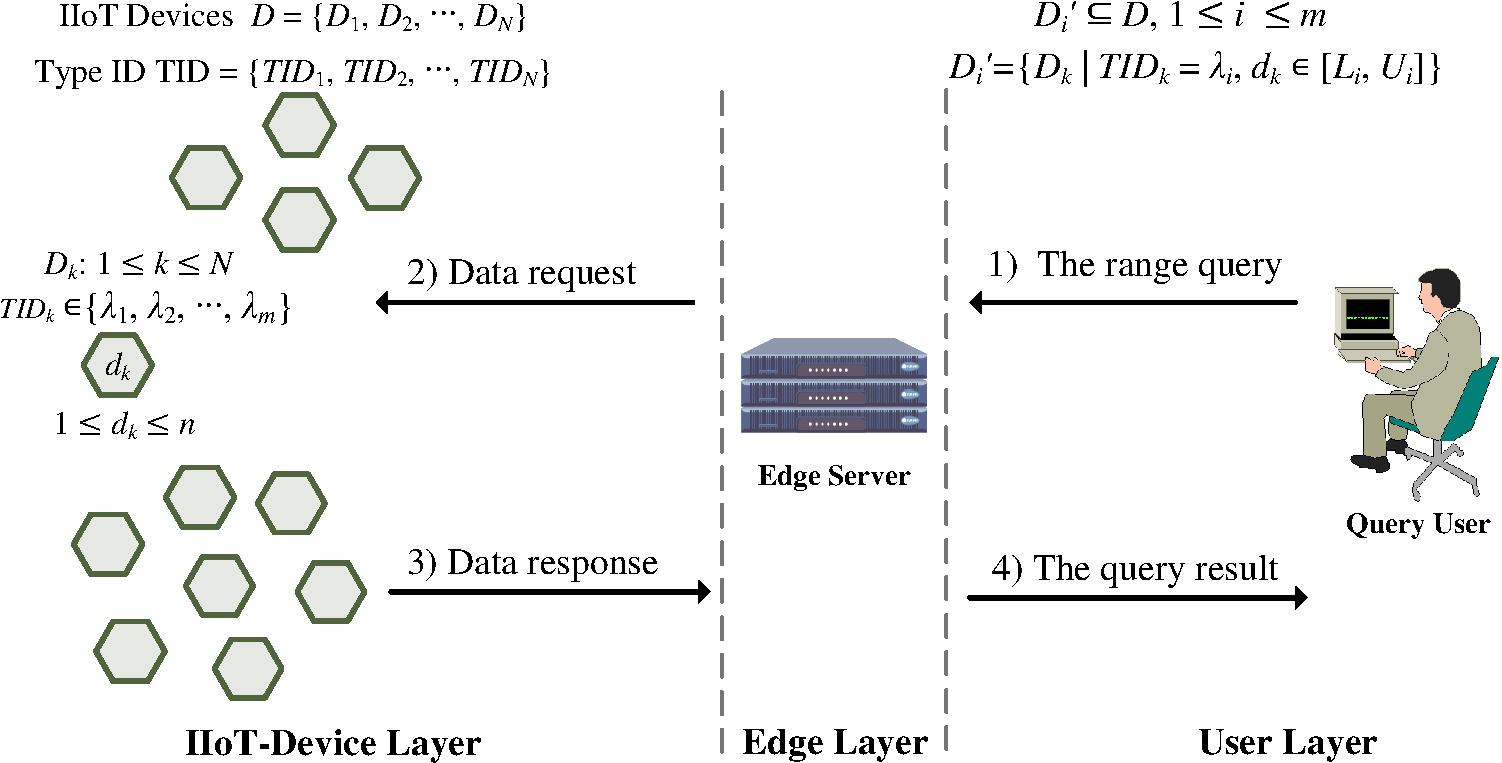
\includegraphics[width=3.3in]{system_model}
  \caption{System model of Edge-PPMRQ}\label{system model}
\end{figure}

\subsection{Security Model}
In Edge-PPMRQ, we assume that all entities are honest-but-curious, i.e., each entity performs the operations according to the protocol, but they also want to reveal the privacy of other entities. For example, IoT devices and the edge server are curious about the query ranges $[L_i, U_i]$ and the corresponding query results $|D'_i|$, where $1 \le i \le m$; the edge server and the query user are also curious about the sensed data $d_k$ of IoT device $D_k$. This paper focuses on  the challenge of the privacy-preserving multi-dimensional range query. Similar to the preview work, we assume that there is no collusion among the entities. Meanwhile, we don't consider active attacks of an external adversary, which will be discussed in future work.

\subsection{Design Goals}
Based on the aforementioned system and security models, a privacy-preserving multi-dimensional range query scheme for edge-supported IIoT should achieve the following goals.
\begin{enumerate}

	\item \emph{Multi-dimensional range query}: Most of traditional range query schemes only support the single-dimensional range query in a query request, while the multi-dimensional range query scheme can realize the query for multi-dimensional data by sending only one query request.

	\item\emph{Privacy-preserving}: The query ranges $[L_i, U_i]$ and the query result $|D'_i|,\ i \in [1, m]$,  cannot be revealed by any other entities except the query user. Besides, the edge server and the query user not only cannot get IoT devices' plaintext of sensed data, but also cannot determine the if the sensed data of IoT devices is within the query ranges.
	
	\item \emph{Continuous, discontinuous and arbitrary boundary range query}:
	Most of the traditional range query schemes only support continuous range query, while in reality, the query ranges may be discontinuous and arbitrary boundary. Consequently, it is very necessary for the multi-dimensional range query schemes to support all the three types of range queries.
	 
	\item \emph{Communication and computationally efficient}: Compared to achieving multi-dimensional range query via single-dimensional range query schemes, a multi-dimensional range query scheme should significantly improve the efficiency of communication and computation. Especially, in edge-supported IIoT, the communication and computation loads of IoT side should be minimized as much as possible.
\end{enumerate}

\section{The Proposed Scheme: Edge-PPMRQ}
In this section, we introduce a privacy-preserving multi-dimensional range query scheme for edge-supported IIoT (Edge-PPMRQ). Before the detailed description of the scheme, we first present our ranges division algorithm, which is a critical technology in Edge-PPMRQ. Besides, the notations used in Edge-PPMRQ are listed in Table \ref{Notations}.

\begin{table}[h]
	\centering\caption{Notations}
	\label{Notations}
	\begin{tabular}{ll} %% this creates two columns
		\hline
		Notation           & Description\\
		\hline
		$N$                & The number of IoT devices\\
		$n$                & The maximum value of IoT devices' sensed data \\
		$d$                & The data example, which is a value between $1$ and $n$\\
		$D_k, d_k$         & The $k$-th IoT device and its sensed data, $1 \le k \le N$ \\
		$m$                & The number of query dimensions  \\
		$t$                & The number of query sub-ranges  \\
		$\lambda_i$        & The index of $i$-th dimension\\
		$\lambda$          & The set of $\lambda_i$\\
		$TID_i$            & The dimension identifier of $D_i$'s sensed data\\
		$TID$              & The set of $TID_i$\\
		$[L_i, U_i]$       & The query range for $i$-th dimension data\\
		$[l_j, u_j]$       & The $j$-th query sub-range \\
		$D'_i$             & The set of IoT devices, whose sensed data is in $[L_i, U_i]$\\
		$BF_j$  		   & The $j$-th bloom filter \\
		$BF$               & The set of bloom filters\\
		$P_f$              & The false positive rate of $BF$\\
		$E_{ij}(r)$        & The cipher of $\lambda_i$'s tab corresponding to $BF_j$, $r\in\{0, 1\}$\\
		$EM$             & The set of $E_{ij}(r)$\\
		$C_{ij}$           &  The $\lambda_i$'s counter corresponding to $BF_j$\\
		$C$                & The set of $C_{ij}$\\
		$\kappa$           & The security parameter to establish OU encryption\\
		$pk, sk$           & The public key and private key of OU encryption\\
		$s$                & The number of elements mapped into bloom filter\\
		$s_j$              & The length of sub-range $[l_j, u_j]$ \\ 
		$p$ 			   & A large prime number\\
		$g$ 			   & A primitive root of $Z^{*}_p$\\
		$a, g^a$ 		   & The query user's private and public parameters\\
		$b, g^b$ 		   & The IoT devices' private and public parameters\\
		$g^{ab}$           & The key shared among query user and IoT devices\\
		$h$                & A public hash function\\
		$h_k$              & The keyed hash value of $d_k$, i.e., $h(g^{ab} \| d_k)$\\
		\hline
	\end{tabular}
\end{table}


\subsection{Ranges division algorithm}\label{sections division}
In order to achieve the multi-dimensional range query, multi-dimensional query ranges should be processed by the ranges division algorithm as the following steps. 
\begin{enumerate}
	\item \emph{Query bounds extraction:} Suppose that $[L_1, U_1]$, $ [L_2, U_2],... ,$ and $[L_m, U_m]$ represent the query ranges of $m$ dimensions $\lambda_1, \lambda_2, ... ,$ and $\lambda_m$, respectively. For $\forall i$ $\in$ $ [1, m]$, we have $ 1 \le L_i \le U_i \le n$. Then, all the lower bounds and upper bounds are extracted to a set $Q_1=\{L_1 , U_1, L_2, U_2, ... , L_m, U_m\}$. After that, both the minimum value 1 and maximum value $n$ are inserted into $Q_1$. Finally, $Q_1=\{1, L_1 , U_1, L_2, U_2, ... , L_m, U_m, n\}$.
	\item \emph{Query bounds sort}: In order to make the ranges division easier, the set $Q_1$ is sorted from smallest to largest and the repeated bounds are deleted. Finally, a sorted set $Q_2=\{l_1, l_2, ... , l_t, l_{t+1}\}$ is generated, where $l_1=1, l_{t+1}=n, l_j < l_{j+1}$ and $j \in [1, t]$.
	\item \emph{Query sub-ranges generation:} According to $Q_2$, $t$ sub-ranges are generated, i.e., $[l_1, l_2]$, $[l_2, l_3]$, $... $, and $[l_t, l_{t+1}]$. For clarity, we denote the sub-ranges as $[l_1, u_1]$, $[l_2, u_2]$, $... $, and $[l_t, u_t]$. Furthermore, the bounds should be adjusted by adding $1$, subtracting $1$ or remaining unchanged to get final sub-ranges $[l_1', u_1']$, $[l_2', u_2']$, $... $, and $[l_t', u_t'
	]$, and the following two conditions should be satisfied for any query range $[L_i, U_i]$, $1\le i \le m$:
	\begin{enumerate}
		\item $\exists a, b, 1 \le a \le b \le t, [l_a',u_a'] \cup [l_{a+1}', u_{a+1}'] \cup ...  \cup [l_b', u_b'] = [L_i, U_i]$, where $l_a' = L_i$ and $u_b'=U_i$.
		\item $\forall v,w \in [a, b]$, $v \neq w$, $[l_v', u_v']\cap [l_w', u_w'] = \emptyset$. 
	\end{enumerate}	 
	 
\end{enumerate} 
                                             
To better understand our proposed ranges division algorithm, we give a toy example here, which is also shown in Fig. \ref{sections division algorithm}. For $n = 100, m = 2$ and two dimensions $\lambda_1$ and $\lambda_2$ with the corresponding query ranges $[20, 60]$ and $[40, 80]$, respectively, the query sub-ranges can be generated by the above ranges division algorithm:
\begin{enumerate}
	\item According to $[20, 60]$ and $[40, 80]$, we can get $Q_1=\{1, 20, 60, 40, 80, 100\}$.
	\item Based on $Q_1$, we get a sorted set $Q_2=\{1, 20, 40, 60, 80, 100\}$.
	\item Then we can get $5$ sub-ranges $[1, 20], [20, 40], [40, 60],$ $[60, 80]$ and $[80, 100]$. Moreover, the bounds of the sub-ranges are adjusted to generate the final sub-ranges $[1, 19], [20, 39], [40, 60], [61, 80]$ and $[81, 100]$.
	
From the sub-ranges, we can see that:
	\begin{enumerate}
		\item $[20,39] \cup [40, 60] = [20, 60]$ and $[40, 60] \cup [61, 80]=[40, 80]$.
		\item $[20,39] \cap [40, 60] = \emptyset$ and $[40, 60] \cap [61, 80]= \emptyset$.
	\end{enumerate}  
\end{enumerate}

\begin{figure}
	\centering
	% Requires \usepackage{graphicx}
	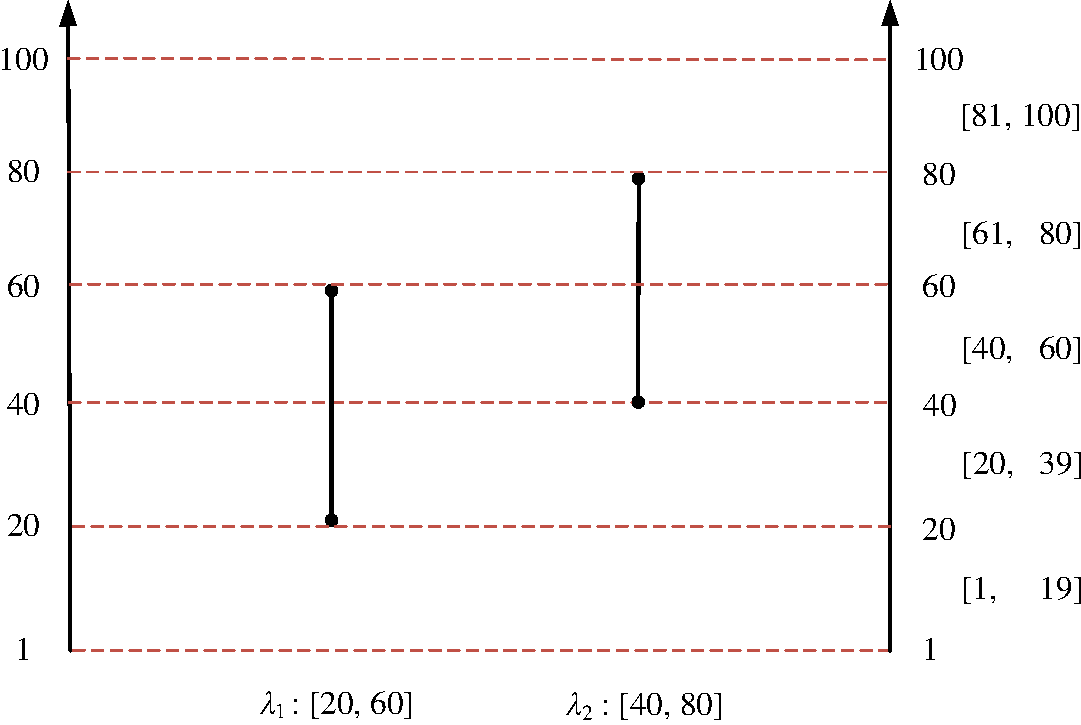
\includegraphics[width=3.4in]{ranges_division_model}\\
	\caption{An example of ranges division algorithm}\label{sections division algorithm}
\end{figure}


\subsection{Description of Edge-PPMRQ}
We now describe our privacy-preserving multi-dimensional range query scheme for edge-supported IIoT (Edge-PPMRQ) in detail by using bloom filter data structure, OU encryption and ranges division algorithm. The five phases of Edge-PPMRQ are illustrated as below. 

\subsubsection{System initialization}
To initialize the system, the service provider selects a hash function $h$, a large prime number $p$, a primitive root $g\in Z^*_p$ and a random number $b\in Z^*_p$. Then, $g^b$ mod $p$ can be computed accordingly. Finally, the service provider publishes the parameters $h, p, g$ and $g^b$. After that, the service provider deploys an edge server and various dimensions IoT devices to the target industrial environment.

\subsubsection{User query request generation}
The query user launches a query for data of $m$ dimensions $\lambda =\{\lambda_1, \lambda_2, ... , \lambda_m\}$, i.e., ``How many IoT devices of dimension $\lambda_i$, whose sensed data $d_k$ is within the range $[L_i, U_i]$, where $1 \le i \le m$ and $1 \le k \le N$?"  In other words, the query user would like to figure out: For $\forall i \in [1, m]$ and $ k \in [1, N]$, $|D_i'|=Count(D'_i)$, where $D'_i=\{D_k | TID_k=\lambda_i$, $d_k \in [L_i, U_i]\}$. To generate the query request in a privacy-preserving way, the query user performs the following steps.

\textbf{Step 1}: Given a security parameter $\kappa$, OU key generation algorithm outputs public key $pk$ and private key $sk$. Besides, a random number $a\in Z_p^*$ is chosen to compute $g^a$ mod $p$ and $g^{ab}=(g^b)^a$ mod $p$, according to the public parameters $p,g$ and $g^b$.
	
\textbf{Step 2}: For $m$ query ranges $[L_1, U_1], [L_2, U_2], ... ,$ and $[L_m, U_m]$ corresponding to dimensions $\lambda_1, \lambda_2, ...,$ and $\lambda_m$, respectively, the ranges division algorithm is called to output $t$ query sub-ranges $[l_1, u_1], [l_2, u_2], ... ,$ and $[l_t, u_t]$. 

\textbf{Step 3}: A group of $t$ bloom filters with $n$-bit vectors and $k$ hash functions are chosen. Here, for each bloom filter, $s$, i.e. the number of mapped elements, should satisfy $s \le \lceil \frac{n}{{\rm log}n} \rceil $ and $k$ should meet $k=\frac{n}{s}{\rm ln}2$ to ensure the false positive rate $P_f=(1-(1-\frac{1}{n})^{ks})^k \approx (1-e^{-\frac{ks}{n}})^k  =n^{-{\rm ln}2}$.

\textbf{Step 4}: For each sub-range $[l_j, u_j]$, $1<j<t$, all integers between $l_j$ and $u_j$ are mapped into $BF_j$. Note that, we don't map the integer value $d\in [l_j, u_j]$ itself but its keyed hash value $h(g^{ab}\|d)$ into $BF_j$. Finally, the sub-ranges $[l_1, u_1], [l_2, u_2], ... ,$ and $ [l_t, u_t]$ are mapped into $t$ bloom filters $BF_1, BF_2, ...,$ and $ BF_t$, respectively. For sub-range $[l_i, u_i]$ with length $s_i$, where $1 \le i \le t$, if $s_i  >\lceil \frac{n}{{\rm log} n} \rceil$, we divide it into some shorter sub-ranges to ensure the false positive rate. For simplicity, we assume that the length $s_i$ is smaller than $\lceil \frac{n}{{\rm log} n} \rceil$.

\textbf{Step 5}: For dimension $\lambda_i$, the query user constructs a query set $\{BF_j, E_{ij}(r), C_{ij}\}$, where $i\in [1, m]$, $j \in [1, t]$ and $r \in \{0, 1\}$. $BF_j$ is the bloom filter which the $j$-th sub-range $[l_j, u_j]$ is mapped into. $E_{ij}(r)$ is the OU ciphertext of $r$, where $r$ is a label to indicate the relationship between the $i$-th dimension $\lambda_i$ and the $j$-th bloom filter $BF_j$. Concretely, if the $j$-th sub-range $[l_j, u_j]$ (mapped into $BF_j$) is a sub-set of the dimension $\lambda_i$'s query range $[L_i, U_i]$, the $r$ is labeled as $1$ $(E_{ij}(r)=E(1))$; otherwise, $r$ is set as $0$ $(E_{ij}(r)=E(0))$.  $C_{ij}$ is a counter with initial value of $0$, which is used to record how many IoT devices of dimension $\lambda_i$, whose sensed data is in the $j$-th sub-range $[l_j, u_j]$. Finally, we get:
	$$EM = {\left [\begin{array}{cccc}
					E_{11}(r) & E_{12}(r) & \cdots & E_{1t}(r)\\
					E_{21}(r) & E_{22}(r) & \cdots & E_{2t}(r)\\
					\vdots    & \vdots    & \ddots & \vdots\\
					E_{m1}(r) & E_{m2}(r) & \cdots & E_{mt}(r)  
					\end{array} \right] },$$
				
	$$C= \left [
		\begin{array}{cccc}
			C_{11} & C_{12} & \cdots & C_{1t}\\
			C_{21} & C_{22} & \cdots & C_{2t}\\
			\vdots & \vdots  & \ddots & \vdots\\
			C_{m1} & C_{m2} & \cdots & C_{mt}
		\end{array}	
		\right].$$
		
\textbf{Step 6}: As shown in Fig. \ref{query request}, the query user constructs a query request $\{\lambda, BF, EM, C, g^a$ mod $p\}$, where $\lambda=\{\lambda_1, \lambda_2, ..., \lambda_m\}$ and $BF=\{BF_1, BF_2, ..., BF_t\}$. Then the query request is sent to the edge server. Accordingly, the edge server broadcasts $\{\lambda,  g^a$ mod $p\}$ to all IoT devices. 

	\begin{figure}
		\centering
		% Requires \usepackage{graphicx}
		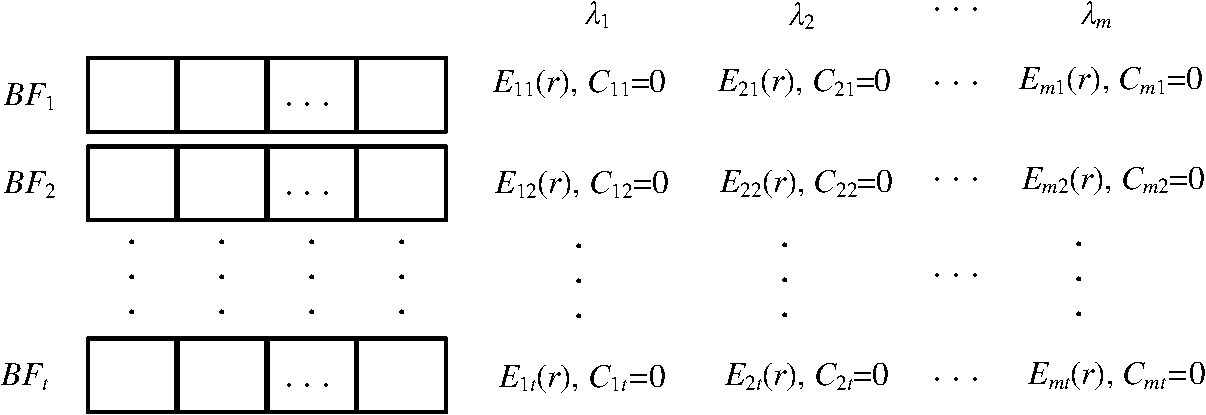
\includegraphics[width=3.4in]{query_request_model}\\
		\caption{Query request generation}\label{query request}
	\end{figure}
	

 Based on the example given in ranges division algorithm, we further show the concrete processes of the user query request generation algorithm:
 	\begin{enumerate}
 		\item For the $5$ sub-ranges $[1, 19], [20, 39], [40, 60] $, $[61 , 80]$ and $[81, 100]$ generated by the ranges division algorithm, we map all the values in the sub-ranges into $5$ bloom filters $BF_1,BF_2,BF_3,BF_4$ and $BF_5$, respectively. For instance, all the values $1, 2, ..., $ and $ 19$ in the sub-range $[1, 19]$ are mapped into $BF_1$.
 		\item For the query range $[20, 60]$ of dimension $\lambda_1$, only $[20, 39]$ and $[40, 60]$ are its sub-sets. Therefore, only the tabs of $E_{12}(r)$ and $E_{13}(r)$ are $1$. Then, the query user constructs a query set $\{BF_j, E_{1j}(r), C_{1j}\}$, $j\in [1, 5]$ and $r \in \{0,1\}$, i.e., $\{\{BF_1, BF_2,BF_3,$ $ BF_4, BF_5\}, \{E_{11}(0),E_{12}(1), E_{13}(1), E_{14}(0), E_{15}(0)\},$ $ \{C_{11}, C_{12}, C_{13}, C_{14}, C_{15}\}\}$. Similarly, for the query range $[40, 80]$ of dimension $\lambda_2$, the query user can also generate the query set correspondingly. Finally, the query request, i.e., the two query sets, is generated as shown in Fig. \ref{query_request_example}.
 	\end{enumerate}
 	
 \begin{figure}
 	\centering
 	% Requires \usepackage{graphicx}
 	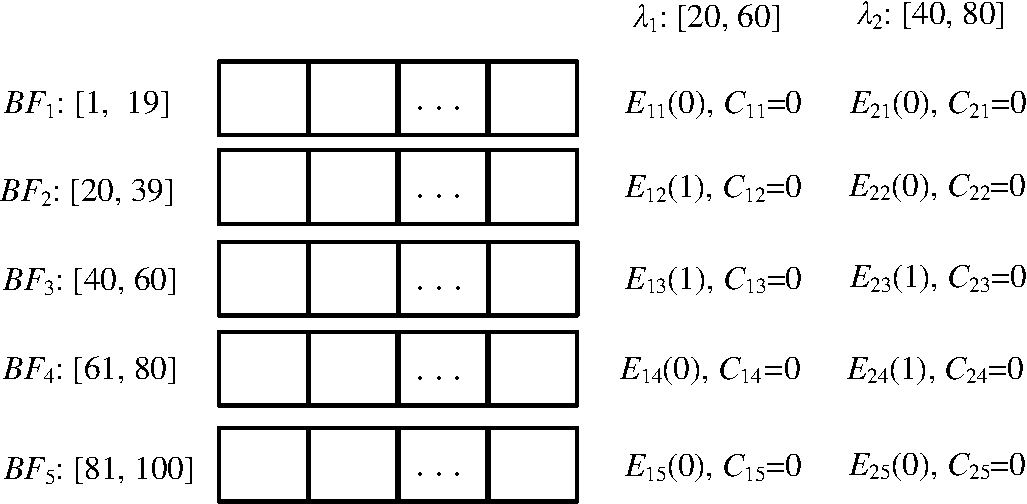
\includegraphics[width=3.4in]{query_request_example}\\
 	\caption{An example of query request}\label{query_request_example}
 \end{figure}

\subsubsection{IoT devices' data response}
 When receiving the data request $\{\lambda,  g^a$ mod $p\}$ forwarded by the edge server, each IoT device $D_k$ $\in D$ checks if its type ID $TID_k$ is in the queried dimensions $\lambda=\{\lambda_1, \lambda_2, ..., \lambda_m\}$. If $TID_k$ doesn't belong to $\lambda$, $D_k$ discards the data request. Otherwise, $D_k$ computes the shared key $g^{ab}$ mod $p$ by using $b$ and $g^a$ mod $p$. Then, $D_k$ computes the
  keyed hash value $h_k=h(g^{ab} \| d_k)$. Finally, $\{TID_k, h_k\}$ is responded to the edge server via a secure channel.

\subsubsection{Edge server data aggregation}
Upon receiving all the responses $\{TID_k, h_k\}, k\in [1, N]$ from IoT devices, the edge server performs the following steps to aggregate the data.

\textbf{Step 1}: Edge server takes $TID_k$ from $\{TID_k, h_k\}$ and find out the corresponding query dimension $\lambda_i$ from $\lambda$, where $1\le i \le m$.  

\textbf{Step 2}: Edge server takes $h_k$ from $\{TID_k, h_k\}$ and checks if $h_k$ is in $BF_j$, where $BF_j \in BF$ and $j \in [1, t]$. If so, the counter $C_{ij}$ increases by $1$. Otherwise, $C_{ij}$ keeps unchanged.

\textbf{Step 3}: After the above processes, the edge server aggregates the data as $C_i = \prod_{j=1}^{t}(E_{ij}(r)^{C_{ij}})$, where $1\le i \le m$, and responses the results $C=\{C_1, C_2, ... ,C_m\}$ to the query user.


  Following the last example, suppose that the data responses from IoT devices are $\{\lambda_1,h(g^{ab}\|5)\},$ $ \{\lambda_1, h(g^{ab}\|20)\},$ $ \{\lambda_1, h(g^{ab}\|30)\},$ $ \{\lambda_2, h(g^{ab}\|35)\},$ $ \{\lambda_2, h(g^{ab}\|45)\}, $ $ \{\lambda_1, h(g^{ab}\|50)\}, $ $ \{\lambda_1, h(g^{ab}\|55)\},$ $ \{\lambda_2, h(g^{ab}\|55)\}, $ $ \{\lambda_2, h(g^{ab}\|65)\}, $ $ \{\lambda_2, h(g^{ab}\|90)\}$. The edge server performs the steps as below to aggregate the sensed data.
   
  \textbf{Step 1}: When receiving the data responses, the edge server sorts the dimension $\lambda_1$'s sensed data $h(g^{ab}\|5), h(g^{ab}\|20),$ $ h(g^{ab}\|30)$, $h(g^{ab}\|50)$ and $h(g^{ab}\|55)$, and $\lambda_2$'s sensed data $h(g^{ab}\|35), h(g^{ab}\|45),$ $ h(g^{ab}\|55), h(g^{ab}\|65)$ and $h(g^{ab}\|90)$. 
  
  \textbf{Step 2}: It checks the bloom filter which the sensed data belongs to and increases the corresponding counter, e.g., $h(g^{ab}\|5)$ of $\lambda_1$ is in $BF_1$, so the corresponding counter $C_{11}$ increases by $1$. Finally, the counters $C_{11}=1, C_{12}=2, C_{13}=2,C_{14}=0, C_{15}=0, C_{21}=0, C_{22}=1, C_{23}=2$, $C_{24}=1$ and $C_{25}=1$.
  
  \textbf{Step 3}: According to $E_{11}(0),E_{12}(1), E_{13}(1),E_{14}(0), E_{15}(0),$ $ E_{21}(0),E_{22}(1), E_{23}(1), E_{24}(0)$ and $E_{25}(0)$ and counters, the data is aggregated as:
  \begin{align*}
  		C_1 &= \prod_{j=1}^{5}(E_{1j}(r)^{C_{1j}})\\
  		    &= E_{11}(0)^{1} \cdot E_{12}(1)^{2} \cdot E_{13}(1)^{2} \cdot E_{14}(0)^{1} \cdot E_{15}(0)^{1} \\
  		    &= E_{11}(0) \cdot E_{12}(2) \cdot E_{13}(2) \cdot E_{14}(0) \cdot E_{15}(0) \\ 
  		    &= E(4)\\
  		C_2 &= \prod_{j=1}^{5}(E_{2j}(r)^{C_{2j}})\\
  		    &= E_{21}(0)^{0} \cdot E_{22}(0)^{1} \cdot E_{23}(1)^{2} \cdot E_{24}(1)^{1} \cdot E_{25}(0)^{1} \\
  		    &= E_{21}(0) \cdot E_{22}(0) \cdot E_{23}(2) \cdot E_{24}(1) \cdot E_{25}(0) \\ 
  		    &= E(3)\\	
  \end{align*}
  Finally, $C=\{C_1, C_2\}$ is replied to the query user.\\
  
	


\subsubsection{User response recovery}
When receiving $C=\{C_1, C_2,$ $ ..., C_m\}$ from the edge server, the query user recovers the corresponding query results $D'=\{|D'_1|, |D'_2|, ... ,|D'_m|\}$ by decrypting $C$ as
\begin{align*}
|D'_i|= Count(D'_i) = Dec(C_i), 1\le i \le m
\end{align*}

The correctness of the result is shown as
\begin{align*}
	Dec(C_i) &= Dec(\prod_{j=1}^{t}(E_{ij}(r)^{C_{ij}})) \\
&= Dec(\prod_{BF_j\in [L_i, U_i]}(E_{ij}(1)^{C_{ij}}) \cdot \prod_{BF_j \notin [L_i, U_i]}(E_{ij}(0)^{C_{ij}})) \\ 
&= Dec(E(\sum_{BF_j \in [L_i, U_i]}(1\cdot C_{ij}) + \sum_{BF_j \notin [L_i, U_i]}(0\cdot C_{ij}))) \\
&= Dec(E(\sum_{BF_j \in [L_i, U_i]}C_{ij})) \\
\end{align*}\begin{align*}
&= \sum_{BF_j \in [L_i, U_i]}C_{ij}\ \ \ \ \ \ \ \ \ \ \ \ \ \ \ \ \ \ \ \ \ \ \ \ \ \ \ \ \ \ \ \ \ \ \ \ \\\
&= |D'_i|.
\end{align*}

In our example, when receiving $C=\{C_1, C_2\}$, the query user can recover the query result as:
 \begin{align*}
 |D'_1| &= Count(D'_1) = Dec(C_1)=4. \\
 |D'_2| &= Count(D'_2) = Dec(C_2)=3. 
 \end{align*}
 
 Therefore, the query user knows that there are $4$ sensed data of dimension $\lambda_1$ in the query range $[20, 60]$ and $3$ sensed data of dimension $\lambda_2$ in the range $[40, 80]$.

\section{Security Analysis}
In this section, we analyze the security features of Edge-PPMRQ and prove that it achieves the aforementioned security requirements. We especially focus on privacy-preserving properties as below.

\begin{enumerate}
	\item \emph{Query ranges $[L_i, U_i], i\in [1, m]$ are privacy-preserving in Edge-PPMRQ}:
	In order to achieve multi-dimensional range query, the $m$-dimensional query ranges are divided into $t$ sub-ranges by the proposed ranges division algorithm. Then the sub-ranges are mapped into $t$ bloom filters to generate the query request. Subsequently, the query request is transferred to the edge server by the query user via a public channel. Through the channel, an IoT device $D_k$ can eavesdrop the query request. At the same time, $D_k \in D$ owns shared key $g^{ab}$ mod $p$. Therefore, for $\forall d \in [1, n]$, $D_k$ can compute all keyed hash values $h(g^{ab} \| d)$ and check the bloom filter which $h(g^{ab} \| d)$ belongs to. In such way, $D_k$ can recover the sub-range $[l_j, u_j]$, which is mapped into $BF_j$, $j\in[1, t]$. However, $D_k$ cannot distinguish the ciphertexts of $0$ and $1$ because OU encryption is a semantically secure cryptosystem \cite{ou1998}, i.e., it cannot know the real value of the tab $r$ in $E_{ij}(r)$. As a result, $D_k$ cannot confirm if the query sub-range $[l_j, u_j]$ is a sub-set of the query range $[L_i, U_i]$. Due to the same reason, even though $D_k$ knows sub-range $[l_j, u_j]$ is mapped into $BF_j$, $D_k$ still cannot get any information about the query range $[L_i, U_i]$ of dimension $\lambda_i$. Besides, the edge server not only cannot get shared key $g^{ab}$ mod $p$, but also cannot distinguish the ciphertexts of $0$ and $1$. Therefore, it cannot get any information about $[l_j, u_j]$ and $[L_i, U_i]$. Based on above analysis, the query ranges $[L_i, U_i]$ of dimension $\lambda_i$, $i \in [1, m]$ are privacy-preserving for IoT devices and the edge server in Edge-PPMRQ.
	        
	\item \emph{The query result $D'=\{|D'_1|, |D'_2|, ... , |D'_m|\}$ is also privacy-preserving in Edge-PPMRQ}:
	For the edge server, it receives the query request $\{\lambda, BF, EM, C, g^a$ mod $p\}$ from the query user and the data response $\{TID_k, h_k\}$, $k \in [1, N]$, from IoT devices. Even though it can know the bloom filter which the keyed hash value $h_k=h(g^{ab} \| d_k)$ belongs to, 
	it cannot confirm if a sub-range $[l_j, u_j]$, which is mapped into the bloom filter $BF_j$, is the sub-set of the query range $[L_i, U_i]$ due to the fact that it cannot distinguish the ciphertexts of $0$ and $1$, according to the semantic security of OU cryptosystem \cite{ou1998}.
    Therefore, the edge server cannot confirm if the sensed data $d_k$ of IoT device $D_k$ is in the query range $[L_i, U_i]$ of dimension $\lambda_i$, $i\in [1, m]$, i.e., it has no idea about that how many IoT devices whose sensed data is in range $[L_i, U_i]$. In other words, the query result $D'$ is privacy-preserving for the edge server. Besides, each IoT device $D_k \in D$ owns $g^{ab}$ mod $p$ and can compute all keyed hash values of data in $[1, n]$. However, every IoT device transfers its data response via a secure channel. As a result, $D_k$'s sensed data $d_k$ cannot be recovered by other IoT devices. At the same time, $E_{ij}(r)$ is also indistinguishable for IoT devices. Thus, IoT devices have no way to know the query result $D'$. Based on the above analysis, we prove that the query result $D'$ is privacy-preserving for the edge server and IoT devices.
	
	\item \emph{Plaintext data $d_k$ of IoT device $D_k$ is also privacy-preserving in Edge-PPMRQ}:
	For the edge server, it can get $g^a$ mod $p$ from the query request. However, $b$ is the private parameter of IoT devices. Therefore, the edge server cannot compute $g^{ab}$ mod $p$. In other words, it cannot recover $d_k$ from $h_k=h(g^{ab}\| d_k)$. Similar to some previous work, in our model, the IoT devices send their data response via a secure channel. As a result, $D_k$'s sensed data $d_k$ cannot be recovered by other IoT devices. Likewise, the query user also cannot recover the sensed data of IoT devices. Based on the above analysis, the plaintext data $d_k$ of IoT device $D_k$ is also privacy-preserving.
\end{enumerate}


\section{Performance Evaluation}

In this section, we evaluate the performance of Edge-PPMRQ and three related work, i.e., BFPRQ \cite{mahdikhani2020IoT}, CEPRQ \cite{hasan2020IoT} and URPRQ \cite{mahdikhani2020using} from the aspects of communication overhead and computational costs. Then, we compare these schemes in detail. Here, it should be noted that Edge-PPMRQ and BFPRQ \cite{mahdikhani2020IoT} are based on OU encryption \cite{ou1998} and Paillier encryption \cite{paillier1999}, respectively, while CEPRQ \cite{hasan2020IoT} and URPRQ \cite{mahdikhani2020using} are based on their own constructed homomorphic encryption SHE. All the schemes are simulated with Python 3.8, Gmpy 2 and Math library. The experiments are carried out on an Intel(R) Core (TM) i5-7400 CPU @3.00GHz with Windows 10 system and 24GB RAM. To ensure the fairness, we keep the false positive rate of bloom filters in BFPRQ \cite{mahdikhani2020IoT} and Edge-PPMRQ as $n^{-\rm{ln}2}$. Besides, we simulate $m$-dimensional range query of BFPRQ \cite{mahdikhani2020IoT}, CEPRQ \cite{hasan2020IoT} and URPRQ \cite{mahdikhani2020using} by performing $m$ single-dimensional query requests since they don't support multi-dimensional range query. Furthermore, we evaluate the communication overhead and computational costs of the four schemes in two conditions: (1) $n$ is varying from $2^{10}$ to $2^{20}$, while $m$ is fixed at 16; (2) $m$ is varying from $5$ to $55$, while $n$ is fixed at $2^{20}$. In addition, the detailed parameters setting and notations used in the comparison are shown in Table \ref{parameters table}.

\begin{table}
\centering\caption{The parameters setting and notations}
\label{parameters table}
\begin{tabular}{lll}                                                 
\hline
Parameter & Value \\
\hline
$\kappa$ & $\kappa=512, |p|=|q|=\kappa$\\
$h$ &The public hash function SHA-256\\
$k$ &The number of hash functions $k$= $\rm{log}$$n$$ \times\rm{ln}2$ \\
$N$ &The number of single dimension's IoT devices. $N$=$1000$ \\
$|\lambda_i|$ & The length of dimension index with the length of $6$ bits\\
$m$ & The number of dimensions in the query request\\
$b$ & $\rm{log}$$n$\\
$|E_{paillier}|$ & The length of paillier ciphertext\\
$|E_{SHE}|$ & The length of SHE ciphertext\\
$|E_{OU}|$ & The length of OU ciphertext\\
$|H|$ & The length of SHA-256's output\\
\hline
\end{tabular}
\end{table}


\iffalse
\begin{figure*}[htbp]	
	\centering
	\begin{subfigure}[t]{0.3\textwidth}
		\centering
		\includegraphics[width=1\textwidth]{commu1_m}\\
		\caption{Communication overhead of user side}\label{user side communication}	
	\end{subfigure}
	\quad
	\begin{subfigure}[t]{0.3\textwidth}
		\centering
		\includegraphics[width=1\textwidth]{commu2_m}\\
		\caption{Communication overhead of IoT side}\label{IoT side communication}
	\end{subfigure}
	\caption{Communication overhead comparison with varying $m$}\label{communication_m}
\end{figure*}
\fi


  \begin{table*}
	\caption{Communication overhead between the edge server and the query user with varying $n$}\label{commu_1_n}
	\begin{center}
		\begin{tabular}{ l  l  l  l }
			\hline
			Schemes  & Query request (bits)& Query result (bits)& Total overhead (bits) \\ \hline
			BFPRQ    & $m \cdot [b \cdot (n+|E_{paillier}|)+  |\lambda_i|)]$  & $m \cdot (|E_{paillier}| + |\lambda_i|)$ & $ 16 \cdot b \cdot n + 32768 \cdot b + 32864$ \\ 
			CEPRQ       & $m \cdot [(2+\frac{2\cdot b^3+3\cdot b^2-11\cdot b}{6}) \cdot |E_{SHE}| + |\lambda_i|]$ & $m \cdot (|E_{SHE}| + |\lambda_i|) $ & $ \frac{2560}{3}  \cdot b^4 + \frac{6400}{3} \cdot b^3 + \frac{10240}{3} \cdot b^2 + \frac{124160}{3} \cdot b + 46176 $  \\ 
			URPRQ       & $m \cdot [(b-1) \cdot (b+2) \cdot |E_{SHE}| + |\lambda_i|]$ & $m \cdot (|E_{SHE}|+ |\lambda_i|)$ & $2560 \cdot b^{3} + 2560 \cdot b^{2} + 96$ \\ 
			Edge-PPMRQ  & $b \cdot (n +m  \cdot |E_{OU}|) + m \cdot |\lambda_i| $     &  $m \cdot (|E_{OU}|+ |\lambda_i|)$  & $b \cdot n + 24576 \times b + 24672$ \\ \hline
		\end{tabular}
	\end{center}
\end{table*}


 \begin{table*}
	\caption{Communication overhead between the edge server and the IoT devices with varying $n$}\label{commu_2_n}
	\begin{center}
		\begin{tabular}{ l  l  l  l }
			\hline
			Schemes  & Data request (bits)& Data response (bits)& Total overhead (bits) \\ \hline
			BFPRQ    & $m \cdot |\lambda_i|$  & $m \cdot N \cdot (|H| + |\lambda_i|)$ & $4192096$ \\ 
			CEPRQ       & $m \cdot [(2+\frac{2\cdot b^3+3\cdot b^2-11\cdot b}{6}) \cdot |E_{SHE}| + |\lambda_i|]$ & $m \cdot N \cdot  (|E_{SHE}| + |\lambda_i|)$ & $ \frac{2560}{3}  \cdot b^4 + \frac{6400}{3} \cdot b^3 + \frac{10240}{3} \cdot b^2 + \frac{124160}{3} \cdot b + 46176 $  \\ 
			URPRQ       & $m \cdot [(b-1) \cdot (b+2) \cdot |E_{SHE}| + |\lambda_i|]$ & $m \cdot N \cdot  (|E_{SHE}| + |\lambda_i|)$ & $2560 \cdot b^{3} + 2560 \cdot b^{2} + 96$ \\ 
			Edge-PPMRQ  & $m \cdot |\lambda_i|$   &  $m \cdot N \cdot (|H| + |\lambda_i|)$  & $4192096$ \\ \hline
		\end{tabular}
	\end{center}
\end{table*}



\begin{figure*}%[htbp]	
	\centering
	\begin{subfigure}[t]{0.23\textwidth}
		\centering
		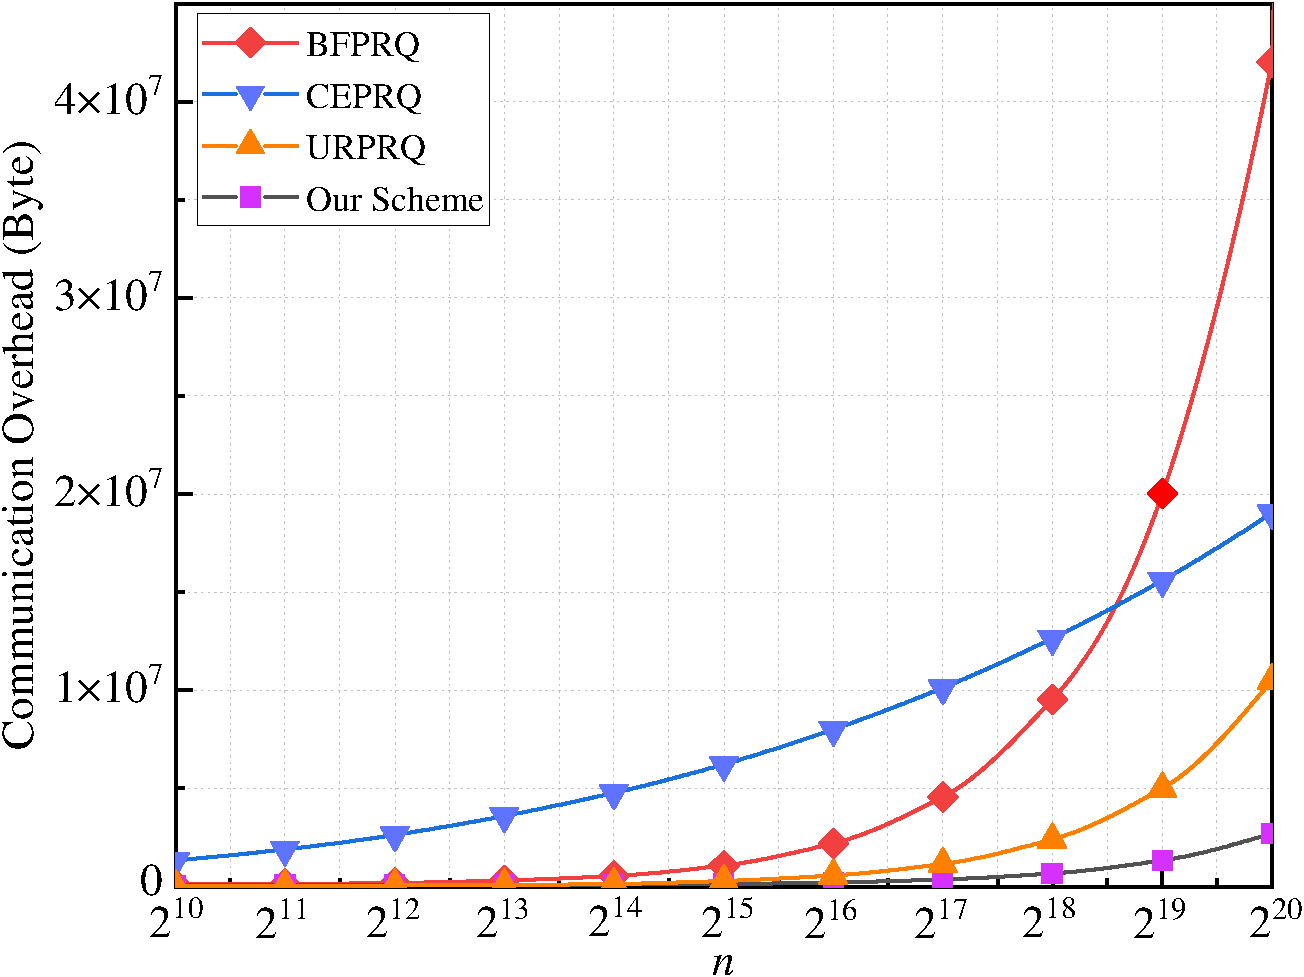
\includegraphics[width=1\textwidth]{commu_1n}\\
		\caption{Between edge server and query user with varying $n$}\label{commu_1n}	
	\end{subfigure}
	\quad
	\begin{subfigure}[t]{0.23\textwidth}
		\centering
		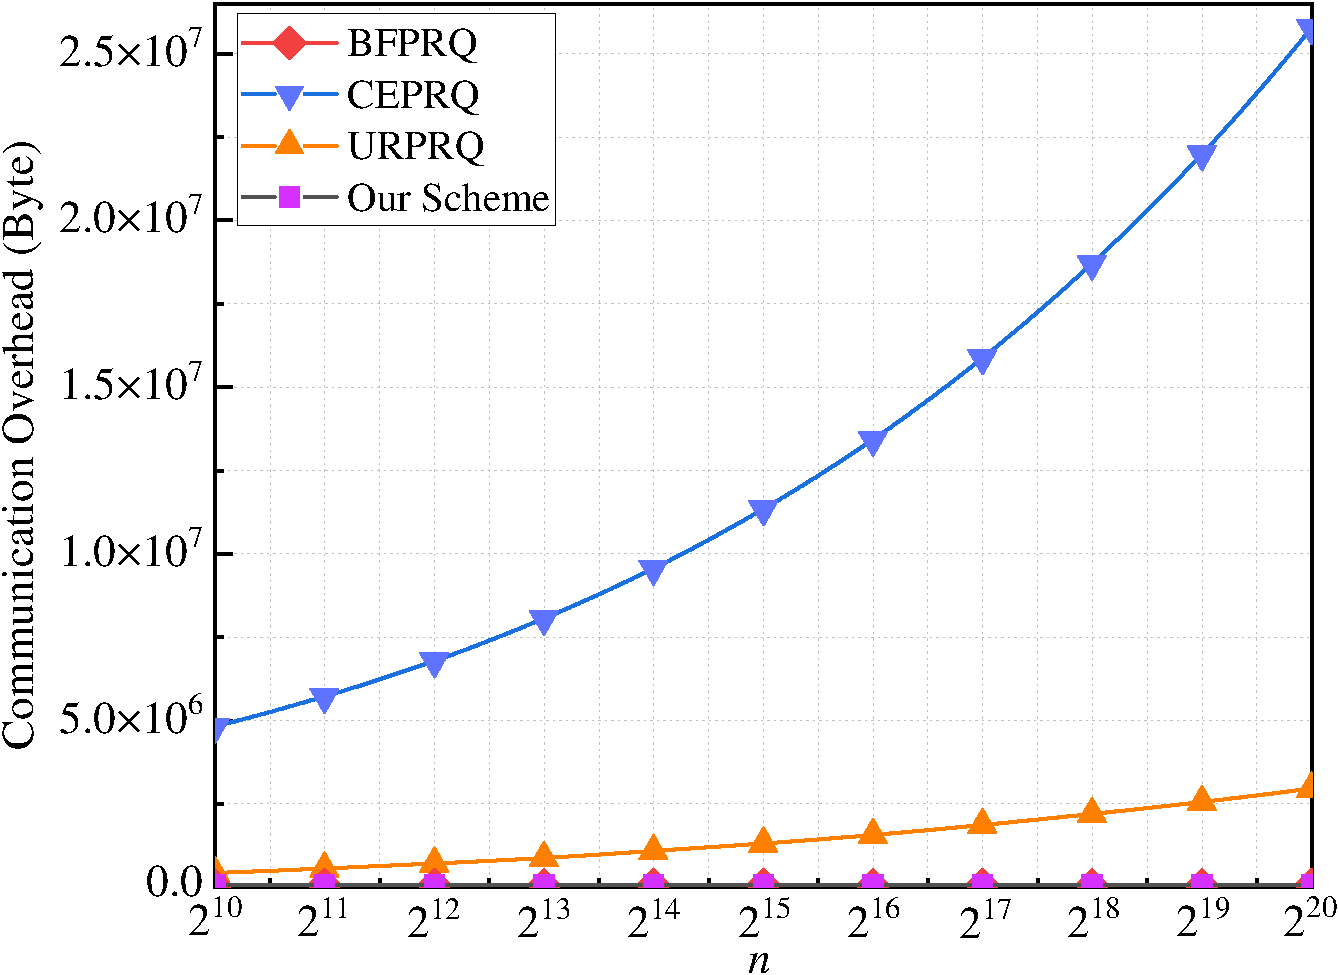
\includegraphics[width=1\textwidth]{commu_3n}\\
		\caption{Between edge server and IoT devices with varying $n$}\label{commu_3n}
	\end{subfigure}
	\quad
	\begin{subfigure}[t]{0.23\textwidth}
		\centering
		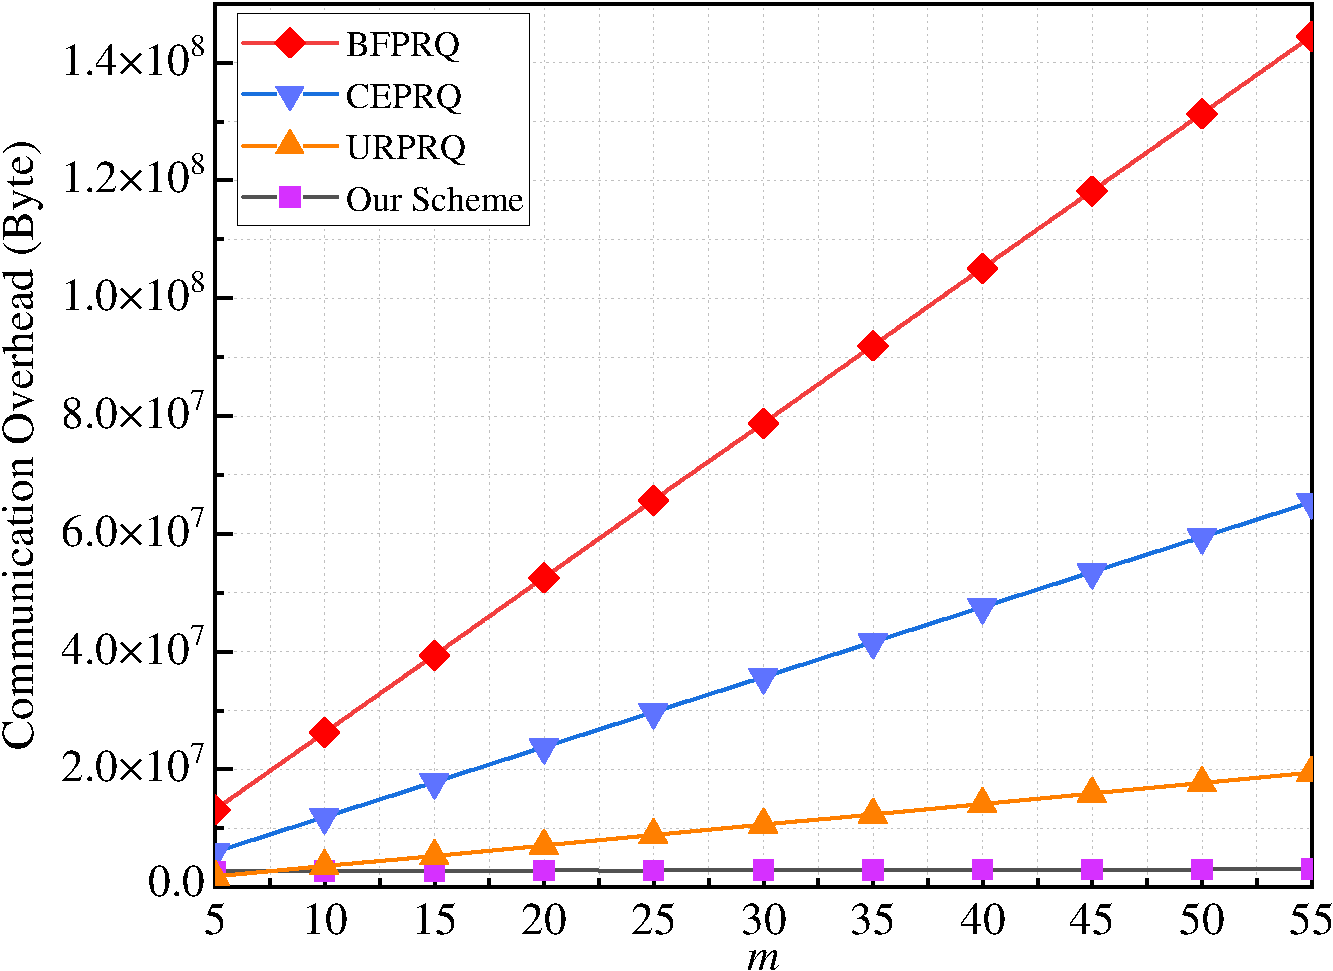
\includegraphics[width=1\textwidth]{commu_1m}\\
		\caption{Between edge server and query user with varying $m$}\label{commu_1m}	
	\end{subfigure}
	\quad
	\begin{subfigure}[t]{0.23\textwidth}
		\centering
		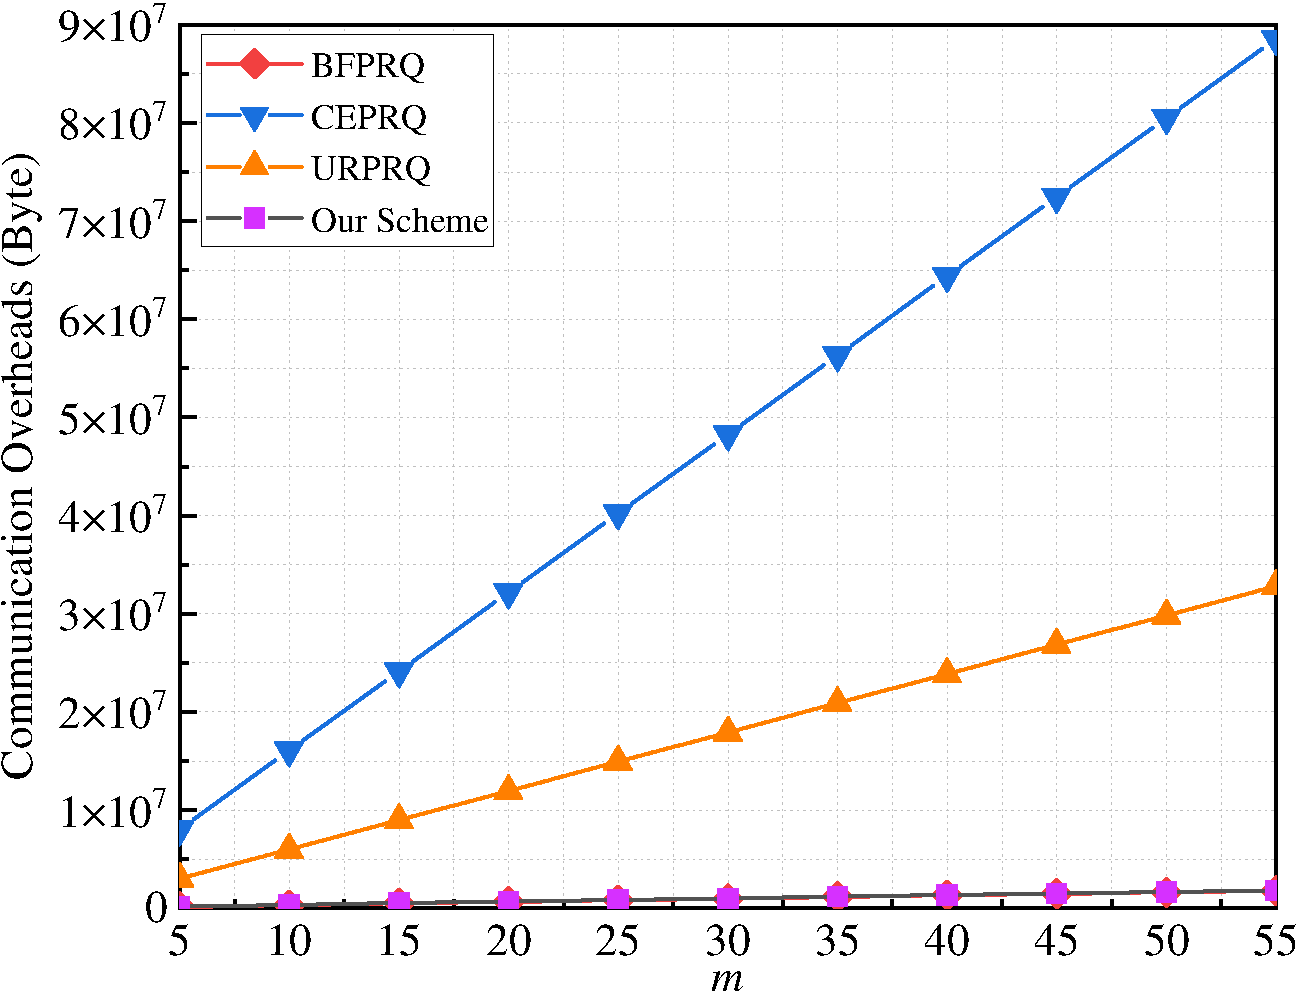
\includegraphics[width=1\textwidth]{commu_3m}\\
		\caption{Between edge server and IoT devices with varying $m$}\label{commu_3m}
	\end{subfigure}
	%\caption{Communication Overhead Comparison with varying $m$}\label{communication}
	\caption{Communication overhead comparison}\label{communication}
\end{figure*}

\subsection{Communication overhead}
In this section, we compare the communication overhead of BFPRQ \cite{mahdikhani2020IoT}, CEPRQ \cite{hasan2020IoT}, URPRQ \cite{mahdikhani2020using} and Edge-PPMRQ. The communication overhead between edge server and query user includes both the query request and query response. Besides, the communication overhead between edge server and IoT devices consists of data request and data response.
  
  For condition 1, we calculate the communication overhead of the four schemes between the edge server and the query user, and between the edge server and IoT devces, which are respectively shown in table \ref{commu_1_n} and table \ref{commu_2_n}.  In order to compare them more intuitively, Fig. \ref{commu_1n} and Fig. \ref{commu_3n} depict the communication overhead in condition 1. From the Fig. \ref{commu_1n}, we can see that the communication overhead between the edge server and the query user in Edge-PPMRQ keeps very low with $n$ varying from $2^{10}$ to $2^{20}$, while in BFPRQ \cite{mahdikhani2020IoT}, CEPRQ \cite{hasan2020IoT} and URPRQ \cite{mahdikhani2020using}, they grow rapidly. Fig. \ref{commu_3n} shows the communication overhead comparison between edge server and IoT devices, from which we can know that both Edge-PPMRQ and BFPRQ \cite{mahdikhani2020IoT} are equally efficient and perform significantly better than CEPRQ \cite{hasan2020IoT} and URPRQ \cite{mahdikhani2020using}. 
  
  
 \iffalse 
  (1) $m\cdot [b \cdot (n+|E_{paillier}|)+  |\lambda_i|)] + m \cdot |E_{paillier}| = 6 \cdot b\cdot(n+2048) + 16 \cdot 2048 +96= 16 \cdot n \cdot b + 32768 \cdot b + 32864$ (bits);   (2) $m \cdot [(2+\frac{2\cdot b^3+3\cdot b^2-11\cdot b}{6}) \cdot |E_{SHE}| + |\lambda_i|] +m \cdot |E_{SHE}| = 16\cdot[(2+\frac{2\cdot b^3+3\cdot b^2-11\cdot b}{6}) \cdot 160 \cdot (b+1) + 16\cdot 6]+ 16 \cdot 160 \cdot (b+1))= 2560/3  \cdot b^4 + 6400/3 \cdot b^3 + 10240/3 \cdot b^2 + 124160/3 \cdot b + 46176 $ (bits);  (3) $m \cdot [(b-1) \cdot (b+2) \cdot |E_{SHE}| + |\lambda_i|] + m \cdot |E_{SHE}| = 16 \cdot [(b-1) \cdot (b+2)\cdot |E_{SHE}|+ 6] + 16 \cdot |E_{SHE}| = 16 \cdot (b-1) \cdot (b+2) \cdot |E_{SHE} | = 2560 \cdot b^{3} + 2560 \cdot b^{2} + 96$ (bits).  (4) $b\cdot (n +m  \cdot |E_{OU}|) + m \cdot |\lambda_i| + m \cdot |E_{OU}| = b\cdot (n + 16 \cdot 1536) + 16 \cdot 1536 + 16 \cdot 6 =b \cdot n + 24576 \cdot b + 24672$ (bits); ,respectively, where $b=\rm{log}_2{n}$. Note that, $m$ is the number of dimensions in the query request. $|E_{paillier}|, |E_{SHE}|, |E_{OU}|$ and $|H|$ are the ciphertext length of paillier, SHE, OU and SHA-256, respectively. 
\fi
  
  
    For condition 2, we also analyze the communication overhead of the four schemes between the edge server and query user, and between the edge server and IoT devces, which are respectively shown in table \ref{commu_1_m} and table \ref{commu_2_m}. Similarly, Fig. \ref{commu_1m} and Fig. \ref{commu_3m} intuitively present the communication overhead of the four schemes in condition 2. From the Fig. \ref{commu_1m}, the communication overhead between the edge server and the query user of the four schemes all show a linear growth trend, but the communication cost curve of Edge-PPMRQ is almost flat with varying $m$ from $5$ to $55$, while the slopes of other schemes, BFPRQ \cite{mahdikhani2020IoT}, CEPRQ \cite{hasan2020IoT} and URPRQ \cite{mahdikhani2020using}, are much greater than that of Edge-PPMRQ. The reason is that Edge-PPMRQ achieves multi-dimensional range query by a query request, which saves a large number of communication cost for multi-dimension query range. Fig. \ref{commu_3m} depicts the communication overhead between the edge server and IoT devices. From the figure, we find that the communication overhead in both Edge-PPMRQ and BFPRQ \cite{mahdikhani2020IoT} keeps efficient, but the communication of CEPRQ \cite{hasan2020IoT} and URPRQ \cite{mahdikhani2020using} are almost $8$ times and $50$ times of that in Edge-PPMRQ, respectively. This is because in CEPRQ \cite{hasan2020IoT} and URPRQ \cite{mahdikhani2020using}, IoT devices not only receive the query request forwarded by the edge server, but also send ciphertext response back, which result in a lot of communication overhead, while IoT devices of Edge-PPMRQ and BFPRQ \cite{mahdikhani2020IoT} only send keyed hash values $h( g^{ab} \| d_k)$ and dimension index $\lambda_i$ to the edge server, which are far shorter than ciphertext. 
    
    
    
    
    
%  (1) $m\cdot b \times (n+|E_{paillier}|)+m \times |E_{paillier}|+ m  \times |\lambda_i| = m \times 20 \times(2^{20} + 2048) + m \times 2048 + m \times 6 = 21014534 \cdot m $ (bits);  
%  (2) $m\times((2+\frac{2\cdot b^3+3 \cdot b^2-11 \cdot b}{6})\times|E_{SHE}|)+m \times |E_{SHE}|+ m \times |\lambda_i|=m \times((2+\frac{2\cdot 20^3+3\cdot 20^2-11\cdot 20}{6}) \times(160\times (20+1))) + m \times 160\times (20+1)+ m \times 6 = 9518886 \cdot m $ (bits);  
% (3) $b\times (n +m\times|E_{OU}|) + m \times |E_{OU}| + m \times |\lambda_i| = 20 \times (2^{20} + m \times 1536 ) + m \times 6 =  30726 \cdot m + 20971520$ (bits);
% (4) $ m \times (b-1) \times (b+2) \times |E_{SHE}| = 418 \times m \times |E_{SHE}|$ (bits), respectively.

   \begin{table*}
 	\caption{Communication overhead between the edge server and the query user}\label{commu_1_m}
 	\begin{center}
 		\begin{tabular}{ l  l  l  l }
 			\hline
 			Schemes  & Query request (bits)& Query result (bits)& Total overhead (bits) \\ \hline
 			BFPRQ    & $m\cdot [b \cdot (n+|E_{paillier}|)+  |\lambda_i|)]$  & $m \cdot (|E_{paillier}| + |\lambda_i|)$ & $21014534 \cdot m $ \\ 
 			CEPRQ       & $m \cdot [(2+\frac{2\cdot b^3+3\cdot b^2-11\cdot b}{6}) \cdot |E_{SHE}| + |\lambda_i|]$ & $m \cdot (|E_{SHE}| + |\lambda_i|) $ & $ 9518886 \cdot m $  \\ 
 			URPRQ       & $m \cdot [(b-1) \cdot (b+2) \cdot |E_{SHE}| + |\lambda_i|]$ & $m \cdot (|E_{SHE}|+ |\lambda_i|)$ & $858124 \cdot m$ \\ 
 			Edge-PPMRQ  & $b\cdot (n +m  \cdot |E_{OU}|) + m \cdot |\lambda_i| $     &  $m \cdot (|E_{OU}|+ |\lambda_i|)$  &  $30726 \cdot m + 20971520$ \\ \hline
 		\end{tabular}
 	\end{center}
 \end{table*}
 
 
 
  \begin{table*}
 	\caption{Communication overhead between the edge server and the IoT devices}\label{commu_2_m}
 	\begin{center}
 		\begin{tabular}{ l  l  l  l }
 			\hline
 			Schemes  & Data request (bits)& Data response (bits)& Total overhead (bits) \\ \hline
 			BFPRQ    & $m \cdot |\lambda_i|$  & $m \cdot N \cdot (|H| + |\lambda_i|)$ & $262000 \cdot m$ \\ 
 			CEPRQ       & $m \cdot [(2+\frac{2\cdot b^3+3\cdot b^2-11\cdot b}{6}) \cdot |E_{SHE}| + |\lambda_i|]$ & $m \cdot N \cdot  (|E_{SHE}| + |\lambda_i|)$ & $ 12881520 \cdot m $  \\ 
 			URPRQ       & $m \cdot [(b-1) \cdot (b+2) \cdot |E_{SHE}| + |\lambda_i|]$ & $m \cdot N \cdot  (|E_{SHE}| + |\lambda_i|)$ & $2048000 \cdot m $ \\ 
 			Edge-PPMRQ  & $m \cdot |\lambda_i|$   &  $m \cdot N \cdot (|H| + |\lambda_i|)$  & $262000 \cdot m$ \\ \hline
 		\end{tabular}
 	\end{center}
 \end{table*}
  

 
%  (1) $m \cdot N \cdot (|\lambda_i| + |H_{SHA3-256}|)= 262000 \cdot m$ (bits); 
%  (2) $m\times((2+\frac{2\cdot b^3+3\cdot b^2-11\cdot b}{6}) \times |E_{SHE}|) +N \times (|\lambda_i| + |E_{SHE}|) = m\times((2+\frac{2\cdot 20^3+3\cdot 20^2-11\cdot 20}{6}) \times 160 \times (20 + 1))  + 1000 \times m \times ( 6 + 160(20+1)) = 12881520 \cdot m $ (bits);
%  (3)  $m \times N \times |E_{SHE}|= 1000 \cdot m \cdot |E_{SHE}|=2048000 \cdot m $
%  (4) $m \times N \times (|\lambda_i| + |H_{SHA3-256}|)= 262000 \cdot m$ (bits), respectively.


  
  Based on the above comparisons, we can conclude that Edge-PPMRQ is remarkably communication-efficient.



\begin{figure*}	
	\centering
	\begin{subfigure}[t]{0.3\textwidth}
		\centering	
		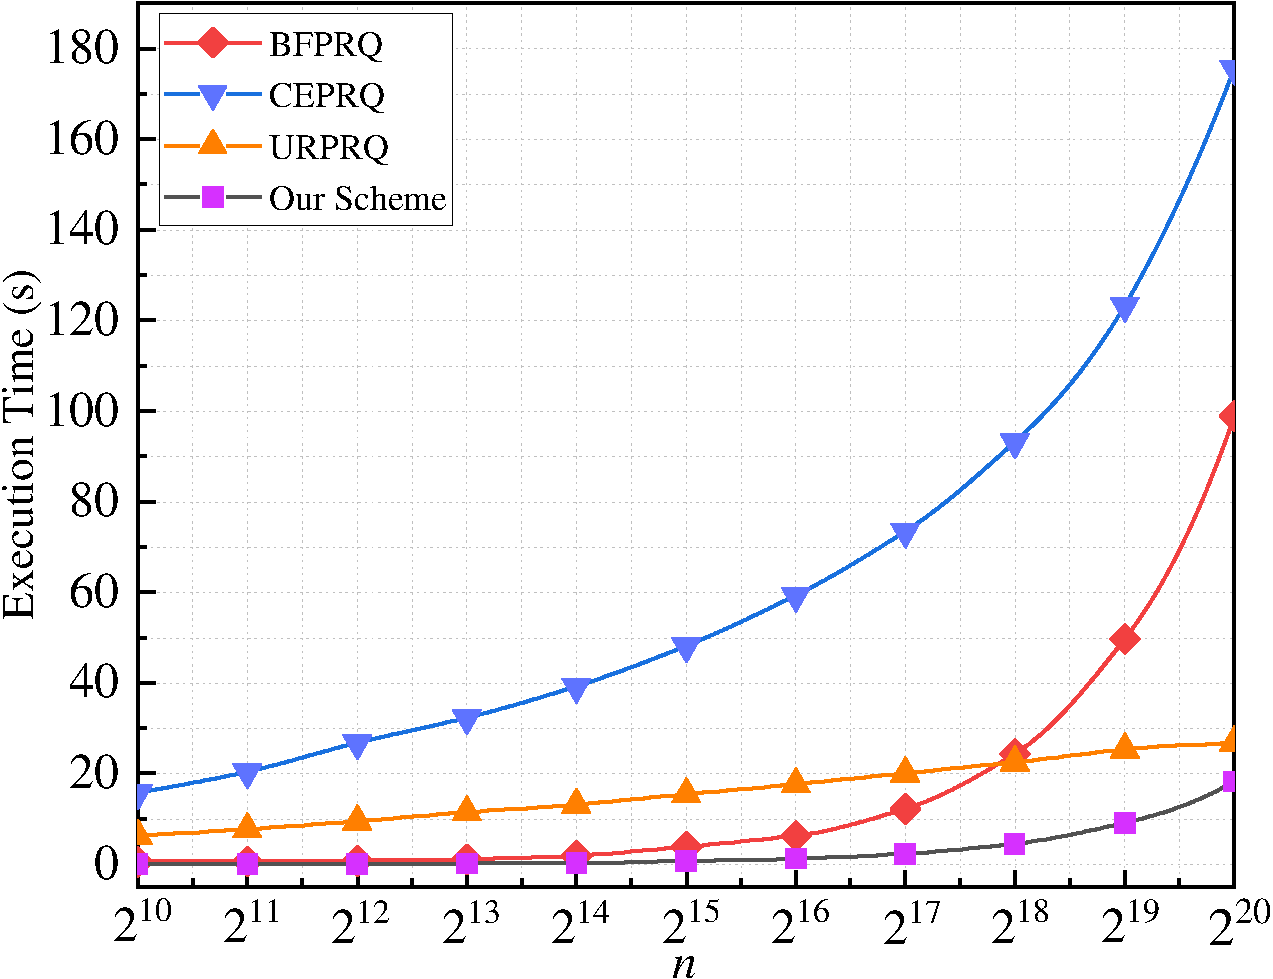
\includegraphics[width=1\textwidth]{com_1n}\\
		\caption{Time cost of user side}
		\label{com_1n}
	\end{subfigure}
	\quad
	\begin{subfigure}[t]{0.3\textwidth}
		\centering
		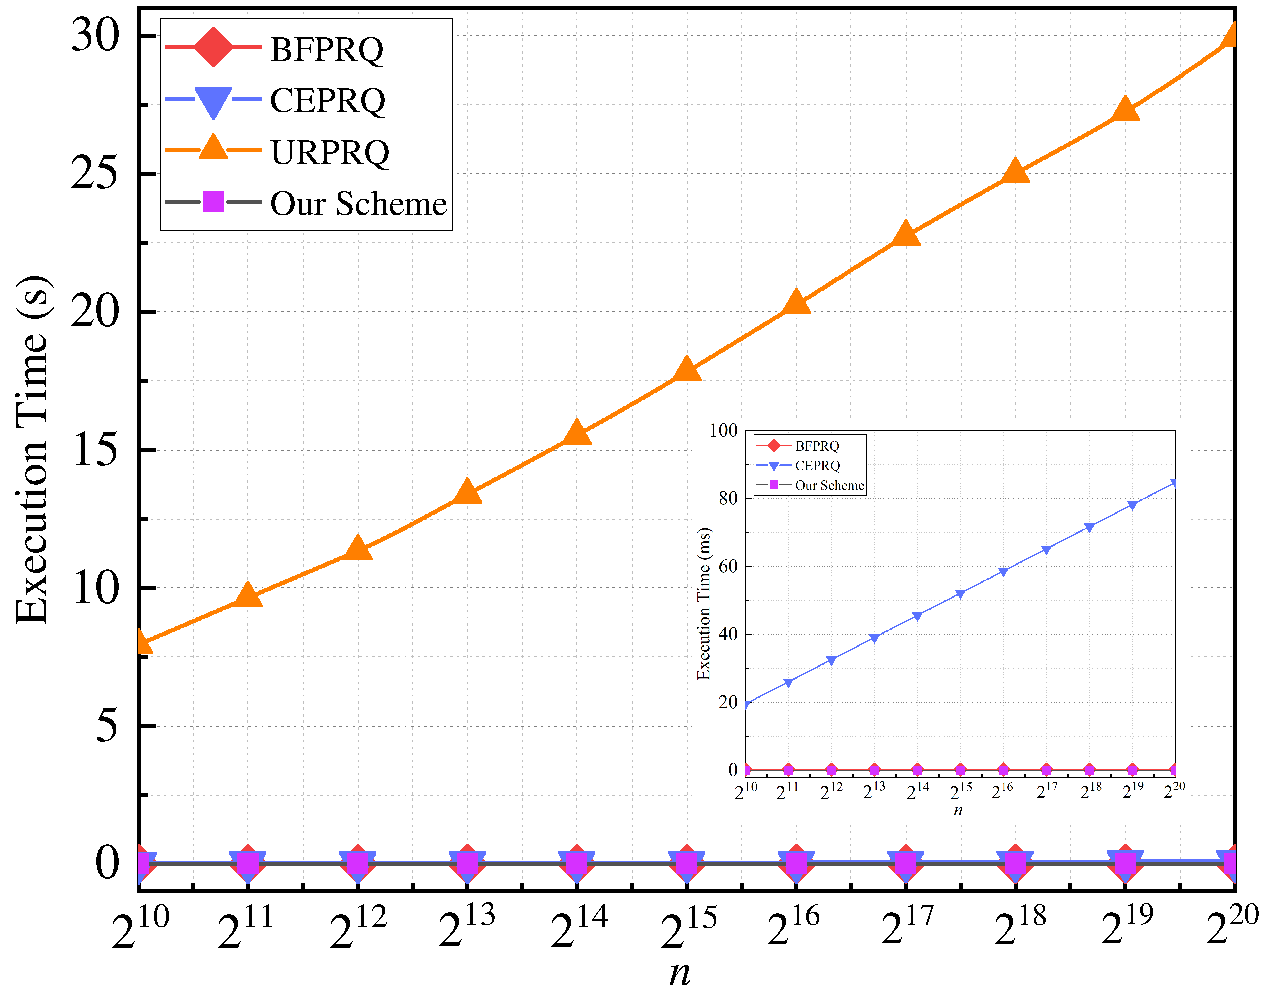
\includegraphics[width=1\textwidth]{com_2n_12}\\
		\caption{Time cost of IoT side}
		\label{com_2n}
	\end{subfigure}
	\quad
	\begin{subfigure}[t]{0.3\textwidth}
		\centering
		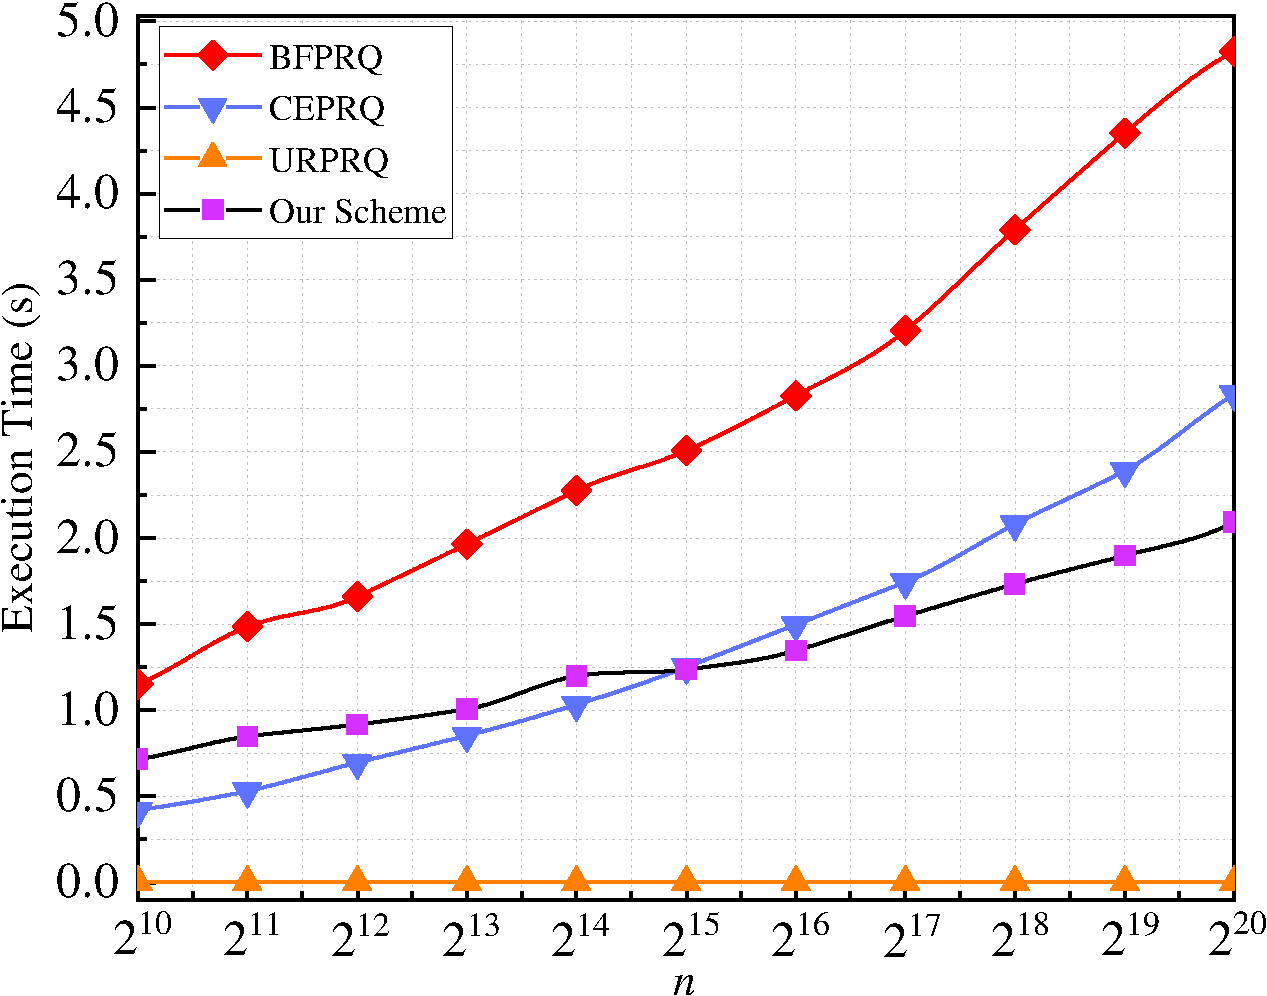
\includegraphics[width=1\textwidth]{com_3n}\\
		\caption{Time cost of edge server side}
		\label{com_3n}
	\end{subfigure}
	\caption{Computational time cost comparison with varying $n$}\label{computation_n}
\end{figure*}

\begin{figure*}%[htbp]	
	\centering
	\begin{subfigure}[t]{0.3\textwidth}
		\centering
		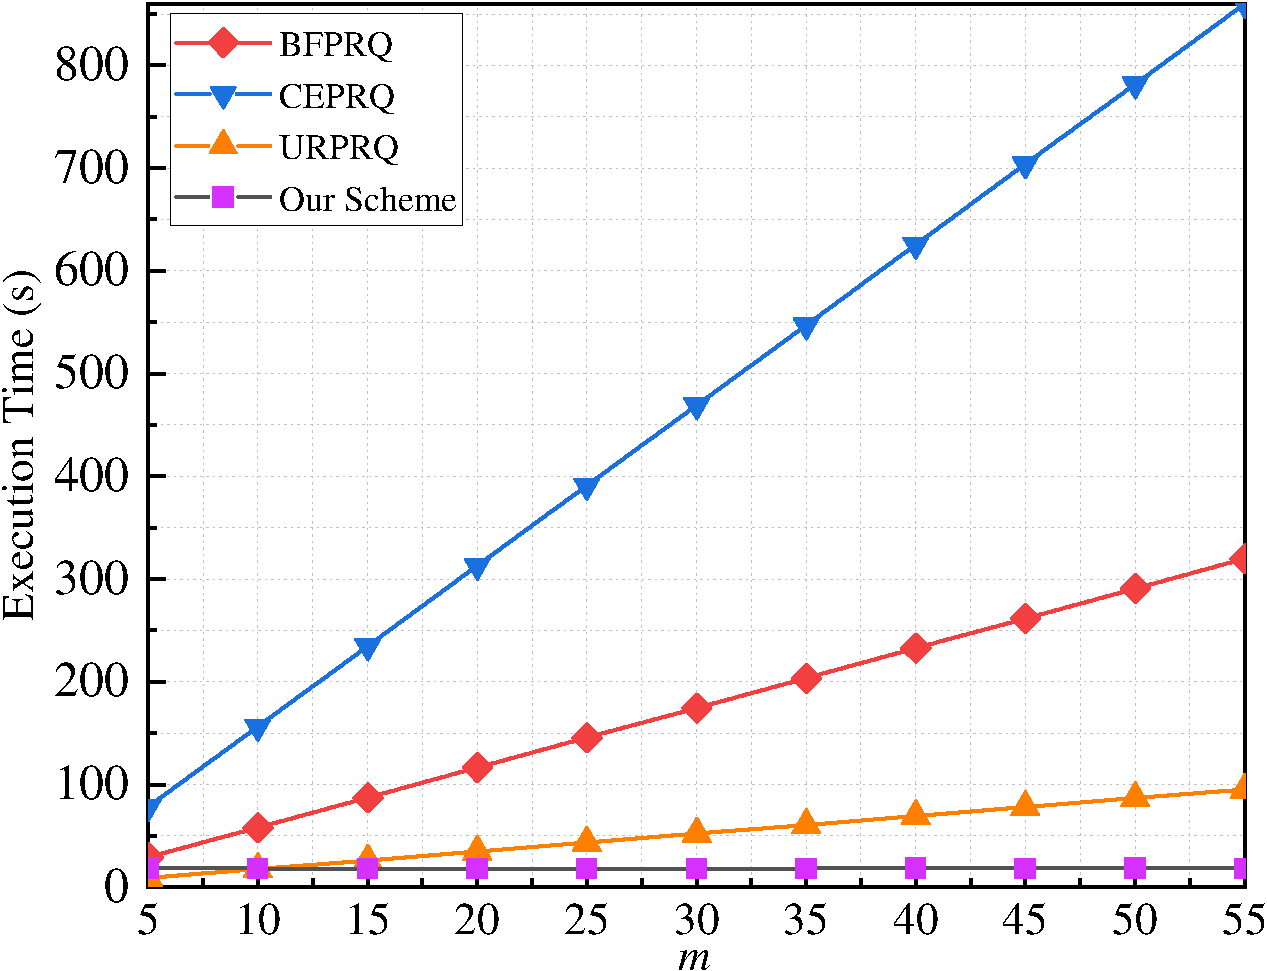
\includegraphics[width=1\textwidth]{com_1m}\\
		\caption{Time cost of user side}\label{com_1m}	
	\end{subfigure}
	\quad
	\begin{subfigure}[t]{0.3\textwidth}
		\centering
		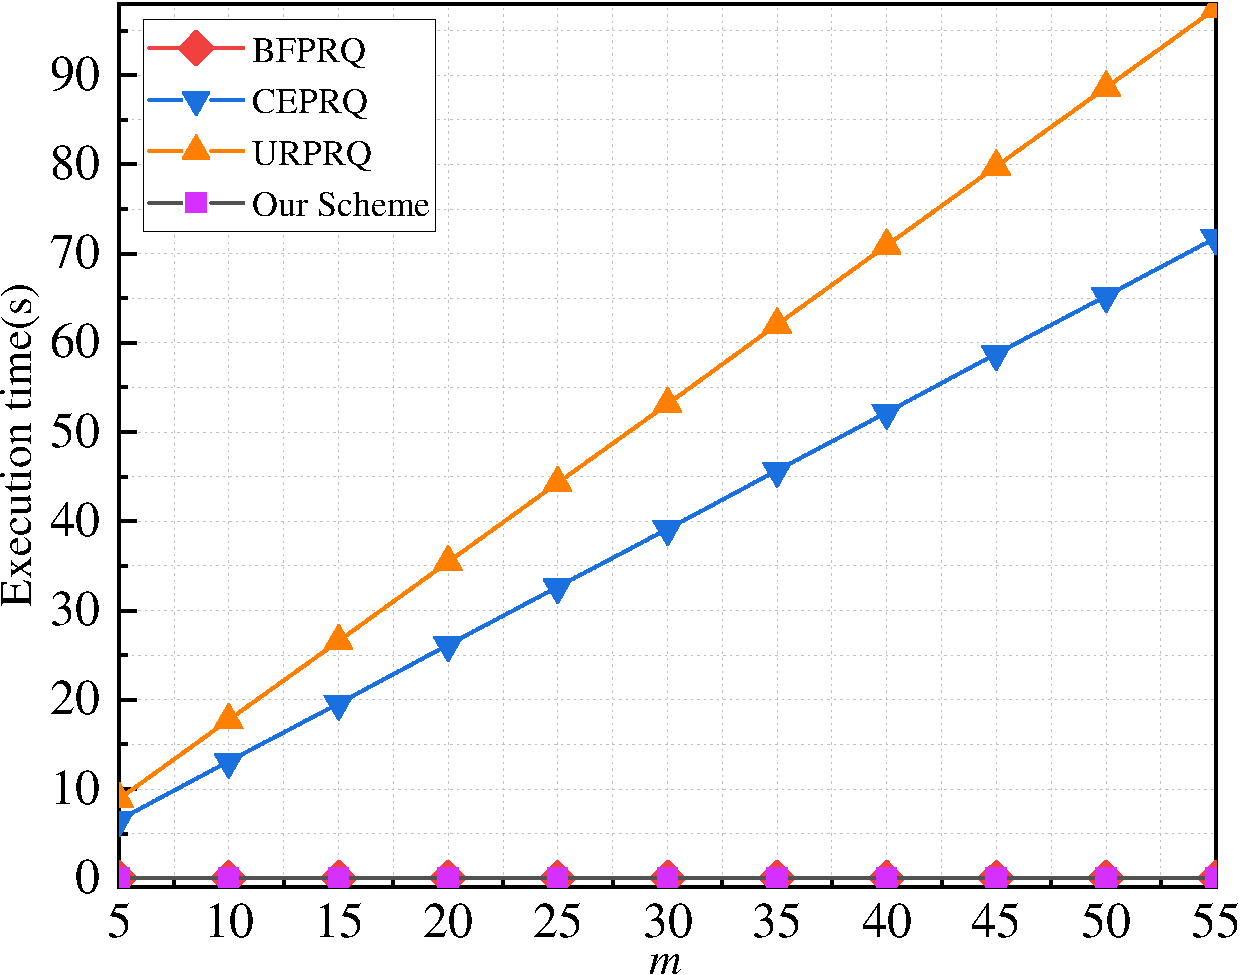
\includegraphics[width=1\textwidth]{com_2m}\\
		\caption{Time cost of IoT side}\label{com_2m}
	\end{subfigure}
	\quad
	\begin{subfigure}[t]{0.3\textwidth}
		\centering
		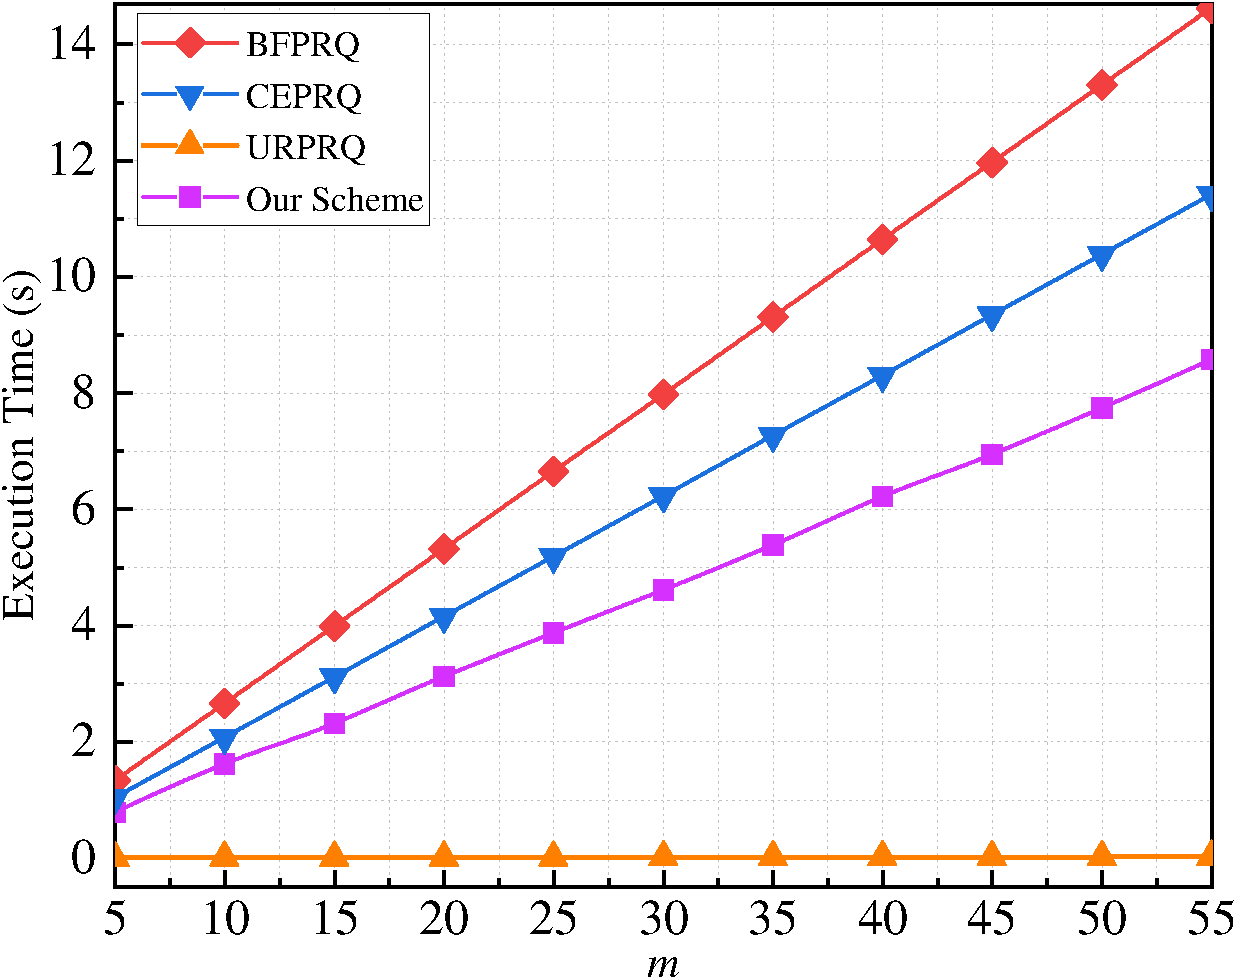
\includegraphics[width=1\textwidth]{com_3m}\\
		\caption{Time cost of edge server side}\label{com_3m}
	\end{subfigure}
	\caption{Computational time cost comparison with varying $m$}\label{computation_m}
\end{figure*}



\subsection{Computational cost}
In this section, we compare the execution time at the query user, IoT devices and the edge server with varying $n$ and $m$, and the experiment comparison results are taken from the average value of 10 times simulations.

Fig. \ref{computation_n} shows the average computational time of BFPRQ \cite{mahdikhani2020IoT}, CEPRQ \cite{hasan2020IoT}, URPRQ \cite{mahdikhani2020using} and Edge-PPMRQ in condition 1. Specifically, Fig. \ref{com_1n} illustrates the execution time of the query user, including user query request generation and user response recovery. From the figure, we can see that Edge-PPMRQ is really efficient, while the execution time of BFPRQ \cite{mahdikhani2020IoT}, CEPRQ \cite{hasan2020IoT} and URPRQ \cite{mahdikhani2020using} increases rapidly with $n$ varying from $2^{10}$ to $2^{20}$. For example, when $n=2^{20}$, the execution time of BFPRQ \cite{mahdikhani2020IoT} and CEPRQ \cite{hasan2020IoT} are $4$ times and $7$ times of that in Edge-PPMRQ, respectively. URPRQ \cite{mahdikhani2020using} also obviously consumes more execution time than Edge-PPMRQ. Fig. \ref{com_2n} shows the execution time at IoT devices. The figure shows that in URPRQ \cite{mahdikhani2020using}, IoT devices undertake a lot of computational costs, while the execution time of other schemes, BFPRQ \cite{mahdikhani2020IoT}, CEPRQ \cite{hasan2020IoT} and Edge-PPMRQ, is negligible. Furthermore, a sub-figure in Fig. \ref{com_2n} is given to better illustrate the comparison among BFPRQ \cite{mahdikhani2020IoT}, CEPRQ \cite{hasan2020IoT} and Edge-PPMRQ. From the sub-figure, we can see that the execution time of CEPRQ \cite{hasan2020IoT} also grows more rapidly than Edge-PPMRQ and BFPRQ \cite{mahdikhani2020IoT}. The reason is that in CEPRQ \cite{hasan2020IoT} and URPRQ \cite{mahdikhani2020using}, IoT devices perform a lot of time-consuming operations, i.e., homomorphic addition and homomorphic xor, while in Edge-PPMRQ and BFPRQ \cite{mahdikhani2020IoT}, IoT devices only compute the keyed hash value, which is much more efficient than homomorphic operations. Fig. \ref{com_3n} indicates the execution time at the edge server. From the figure, we can observe that Edge-PPMRQ, CEPRQ \cite{hasan2020IoT} and URPRQ \cite{mahdikhani2020using} are more efficient than BFPRQ \cite{mahdikhani2020IoT}, and  Edge-PPMRQ performs better than CEPRQ \cite{hasan2020IoT} when $n$ is bigger than $2^{15}$. Although the computational costs of the edge server in URPRQ \cite{mahdikhani2020using} keep very low, it is at the cost of that a large amount of computational overhead for IoT devices  according to Fig. \ref{com_2n}. 


\begin{table*}\centering
	
	\caption{Comprehensive comparison}
	
	\begin{tabular*}{14.7cm}{p{6.5cm}cccc}
		
		\hline
		Schemes & Edge-PPMRQ & BFPRQ \cite{mahdikhani2020IoT} & CEPRQ \cite{hasan2020IoT} & URPRQ \cite{mahdikhani2020using} \\
		\hline
		Multi-dimension             & $\surd$     & $\times$    & $\times$    & $\times$ \\
		Discotinuous range         & $\surd$     & $\surd$  & $\times$  & $\surd$ \\
		Arbitrary boundary range            & $\surd$     & $\surd$  & $\times$  & $\surd$ \\
		Communication overhead between IoT and edge server & low       & low         & middle      & high\\	
		Computational costs in IoT & low        & low         & high	      & high \\
		Computational costs in edge server & middle & high      & middle      & low \\
		\hline
	\end{tabular*}
	\label{comprehensive comparison}
	
\end{table*} 



Fig. \ref{computation_m} depicts the average computational time of BFPRQ \cite{mahdikhani2020IoT}, CEPRQ \cite{hasan2020IoT}, URPRQ \cite{mahdikhani2020using} and Edge-PPMRQ in condition 2. Specifically, Fig. \ref{com_1m} shows the execution time at the query user, including two parts, i.e., user query request generation and user response recovery. We can find that Edge-PPMRQ costs nearly constant execution time, which is apparently efficient than BFPRQ \cite{mahdikhani2020IoT}, CEPRQ \cite{hasan2020IoT} and URPRQ \cite{mahdikhani2020using}. This is because the query user in Edge-PPMRQ performs less homomorphic operations than BFPRQ \cite{mahdikhani2020IoT}, CEPRQ \cite{hasan2020IoT} and URPRQ \cite{mahdikhani2020using}. Fig. \ref{com_2m} depicts IoT devices' data response time, which shows that both Edge-PPMRQ and BFPRQ \cite{mahdikhani2020IoT} are more efficient than CEPRQ \cite{hasan2020IoT} and URPRQ \cite{mahdikhani2020using}. The reason is that IoT devices in Edge-PPMRQ and BFPRQ \cite{mahdikhani2020IoT} only need compute keyed hash values $H( g^{ab} \| d_i)$, while both in CEPRQ \cite{hasan2020IoT} and URPRQ \cite{mahdikhani2020using}, IoT devices need perform a lot of homomorphic multiplication operations. Fig. \ref{com_3m} presents the data aggregation time cost at the edge server, and  Edge-PPMRQ performs better than BFPRQ \cite{mahdikhani2020IoT} and CEPRQ \cite{hasan2020IoT} since in Edge-PPMRQ, the number of homomorphic operations are less than that of BFPRQ \cite{mahdikhani2020IoT} and CEPRQ \cite{hasan2020IoT}. Obviously, URPRQ \cite{mahdikhani2020using} consumes the lowest computational time. The reason is that the most computational costs are afforded by IoT devices, and the edge server only performs cipher homomorphic addition operations.



\subsection{Comprehensive comparison}
Based on above introduce and analysis, a comprehensive comparison of Edge-PPMRQ and related schemes is given in table \ref{comprehensive comparison}.

From a functional point of view, Edge-PPMRQ supports the functions of multi-dimension, discontinuous and arbitrary boundary range query, while BFPRQ \cite{mahdikhani2020IoT}, CEPRQ \cite{hasan2020IoT} and URPRQ  \cite{mahdikhani2020using} cannot support multi-dimension range query. Additionally, CEPRQ \cite{hasan2020IoT} also cannot support discontinuous ranges query and arbitrary boundary range query. 

From a performance perspective, in edge/fog-supported IoT application, the most important mission of edge server/fog node is to reduce the burden of IoT devices, and the most tasks of IoT devices can be migrated to edge server/fog node. As a result, the communication overhead and computational costs of IoT devices can be greatly reduced, which not only remarkably extends the life period of IoT devices, but also achieves nearly real-time service. According to the comparison in the table \ref{comprehensive comparison}, Edge-PPMRQ and BFPRQ \cite{mahdikhani2020IoT} achieve the purpose well, while in CEPRQ \cite{hasan2020IoT} and URPRQ \cite{mahdikhani2020using}, IoT devices takes the most communication and computational tasks. Although BFPRQ \cite{mahdikhani2020IoT} has low communication overhead between IoT devices and the edge server and low computational costs in IoT devices, its computational costs in edge server side is high. CEPRQ \cite{hasan2020IoT} has middle communication overhead between IoT devices and the edge server, and computational costs in the edge server, but it consumes high execution time in IoT devices. Moreover, URPRQ \cite{mahdikhani2020using} not only has high communication overhead between IoT and edge server, but also consumes high computational costs in IoT devices. Although URPRQ \cite{mahdikhani2020using} has lowest computational costs in fog node, it is at the cost of high computational load in IoT devices. Therefore, it is not suitable for edge/fog-supported IoT applications, in which the IoT devices own limited resource. 

In a word, Edge-PPMRQ not only is functionally powerful for multi-dimension, discontinuous and arbitrary boundary range queries, but also achieves communication and computationally efficient for edge-supported IIoT application.

\iffalse
From a performance perspective, in edge/fog-supported IoT application, the most important mission of edge server/fog node is to reduce the burden of IoT devices, and the most tasks of devices can be migrated to edge server/fog node. As a result, the communication overhead and computational costs of IoT side can be greatly reduced. This not only remarkably extends the life period of IoT devices, but also achieves nearly real-time service. According to the comparison in the table \ref{comprehensive comparison}, Edge-PPMRQ and BFPRQ \cite{mahdikhani2020IoT} achieve the purpose well, while in CEPRQ \cite{hasan2020IoT} and URPRQ \cite{mahdikhani2020using}, IoT side takes the most communication and computational tasks. Although BFPRQ \cite{mahdikhani2020IoT} has high computational costs in edge server side and CEPRQ \cite{hasan2020IoT} consumes high execution time in IoT side. Moreover, URPRQ \cite{mahdikhani2020using} not only has high communication overhead between IoT and edge server, but also consumes high computational costs in IoT side. Although URPRQ \cite{mahdikhani2020using} has lowest computational costs in fog node, it is at the cost of high computational load in IoT side, therefore, . 
\fi

\iffalse
More importantly, in edge-supported IoT, fog node and edge server are introduced to employ the most communication and computational costs and support nearly real-time data process. As a result, the communication overhead and computational costs of IoT side can be greatly reduced, which can remarkably extend the life period of IoT side. According to the comparison in the table, Edge-PPMRQ and BFPRQ \cite{mahdikhani2020IoT} achieve the purpose well, while in CEPRQ \cite{hasan2020IoT} and URPRQ \cite{mahdikhani2020using}, IoT side takes the most communication and computational tasks. So, we can conclude that Edge-PPMRQ is the comprehensively best.


Furthermore, in edge/fog-supported IoT application, the most important mission of edge server/fog node is to reduce the burden of IoT devices, and the most tasks of devices can be migrated to edge server/fog node. As a result, the communication overhead and computational costs of IoT side can be greatly reduced. This not only remarkably extends the life period of IoT devices, but also achieves nearly real-time service. According to the comparison in the table, Edge-PPMRQ and BFPRQ \cite{mahdikhani2020IoT} achieve the purpose well, while in CEPRQ \cite{hasan2020IoT} and URPRQ \cite{mahdikhani2020using}, IoT side takes the most communication and computational tasks. Although URPRQ \cite{mahdikhani2020using} has lowest computational costs in fog node, it is at the cost of high computational load in IoT side, the . So, we can conclude that Edge-PPMRQ is the comprehensively best.
\fi

 

\section{Conclusion}
 Based on our proposed ranges division algorithm, this paper has designed a privacy-preserving multi-dimensional range query scheme for edge-supported IIoT. Edge-PPMRQ achieves the function of multi-dimensional range query, i.e. a user can query different types of data at once, which is very suitable for the real application of IIoT environment. Meanwhile, it also supports the continuous, discontinuous and arbitrary boundary range queries. The security analysis proves that Edge-PPMRQ is privacy-preserving, i.e. the query ranges and query results cannot be revealed by any other entities except the query user, and the sensed data of each IoT device cannot be recovered by other parties. Furthermore, a large number of experiments are conducted to evaluate the performance of Edge-PPMRQ and other related work, and the results show that Edge-PPMRQ is really communication and computationally efficient. Comprehensively, Edge-PPMRQ achieves expected goals in aspects of functions, privacy-preservation and efficiency. In future work, we plan to study more efficient range query schemes for various functions, privacy requirements and multiple application scenarios, e.g., multi-user range query scheme.

\footnotesize
\bibliographystyle{IEEEtran}
\bibliography{IEEEabrv,references}
\vspace{12 pt}
\normalsize

\iffalse
\noindent\textbf{Xiong Li} received the Ph.D. degree in computer science and technology from the Beijing University of Posts and Telecommunications, Beijing, China, in 2012. He is currently an Associate Professor with the School of Computer Science and Engineering, Hunan University of Science and Technology, Xiangtan, China. He has authored over 100 referred papers. His current research interests include cryptography and information security. He was a recipient of the 2015 Journal of Network and Computer Applications Best Research Paper Award.\\

\noindent\textbf{Shanpeng Liu}
 is currently a M.S. candidate of Hunan University of Science and Technology, China. His research interests include cloud computing security and security protocols.\\

\noindent\textbf{Fan Wu} received the ME degree in computer software and theory from Xiamen University, Xiamen, China, in 2008. Now, he is an Associate Professor in Xiamen Institute of Technology. His current research interests include information security, internet protocols, and network management.\\

\noindent\textbf{Saru Kumari} received the Ph.D. degree in mathematics from Chaudhary Charan Singh University, Meerut, India, in 2012. She is currently an Assistant Professor in the
Department of Mathematics, Chaudhary Charan Singh University. Her current research interests include information security, digital authentication, and applied mathematics.\\

\noindent\textbf{Joel J.P.C. Rodrigues} (S01, M06, SM06) is a professor and senior researcher at the National Institute of Telecommunications (Inatel), Brazil and senior researcher at the Instituto de Telecomunica\c{c}\~oes, Portugal. Prof. Joel is the leader of the Internet of Things Research Group (Inatel), Director for Conference Development-IEEE ComSoc Board of Governors, and IEEE Distinguished Lecturer. He has authored or coauthored over 650 papers in refereed international journals and conferences, 3 books, and 2 patents. He had been awarded several Outstanding Leadership and Outstanding Service Awards by IEEE Communications Society and several best papers awards.




\vspace{-1cm}
\begin{IEEEbiography}[{\includegraphics[width=1in,height=1.25in,clip,keepaspectratio]{1.jpg}}]{Xiong Li}
received the Ph.D. degree in computer science and technology from the Beijing University of Posts and Telecommunications, Beijing, China, in 2012. He is currently an Associate Professor with the School of Computer Science and Engineering, Hunan University of Science and Technology, Xiangtan, China. He has authored over 100 referred papers. His current research interests include cryptography and information security. He was a recipient of the 2015 Journal of Network and Computer Applications Best Research Paper Award.
\end{IEEEbiography}

\vspace{-1.5cm}
\begin{IEEEbiography}[{\includegraphics[width=1in,height=1.25in,clip,keepaspectratio]{2.jpg}}]{Shanpeng Liu}
 is currently a M.S. candidate of Hunan University of Science and Technology, China. His research interests include cloud computing security and security protocols.
\end{IEEEbiography}
\vspace{-1.5cm}

\begin{IEEEbiography}[{\includegraphics[width=1in,height=1.25in,clip,keepaspectratio]{3.jpg}}]{Fan Wu}
received the ME degree in computer software and theory from Xiamen University, Xiamen, China, in 2008. Now, he is an Associate Professor in Xiamen Institute of Technology. His current research interests include
information security, internet protocols, and network management.
\end{IEEEbiography}
\vspace{-1.5cm}
\begin{IEEEbiography}[{\includegraphics[width=1in,height=1.25in,clip,keepaspectratio]{4.jpg}}]{Saru Kumari}
received the Ph.D. degree in mathematics from Chaudhary Charan Singh University, Meerut, India, in 2012. She is currently an Assistant Professor in the
Department of Mathematics, Chaudhary Charan Singh University. Her current research interests include information security, digital authentication, and applied mathematics.
\end{IEEEbiography}
\vspace{-1.5cm}
\begin{IEEEbiography}
[{\includegraphics[width=1in,height=1.25in,clip,keepaspectratio]{5.jpg}}]{Joel J.P.C. Rodrigues}
[S01, M06, SM06] is a professor and senior researcher at the National Institute of Telecommunications (Inatel), Brazil and senior researcher at the Institute of Telecommunications, Portugal. His research interests contain IoT, Mobile and Cloud Computing and so on. He has authored or coauthored over 500 papers. He is a senior member ACM and IEEE.

\end{IEEEbiography}
\fi


\end{document}


